\section{Sonnenenergie und Baubionik}

\subsection{Sonnenenergie}

\subsubsection{Energietransformation in der Natur}

Ohne Sonne gibt es kein Leben. Primärproduzenten sind Pflanzen, die ihre Energie nur mithilfe von Sonnenlicht durch die Photosynthese herstellen. Elementar wichtig dafür ist der Aufbau der \textbf{Pflanzenzelle}, die aus folgenden Zellorganellen besteht:

\begin{center}
    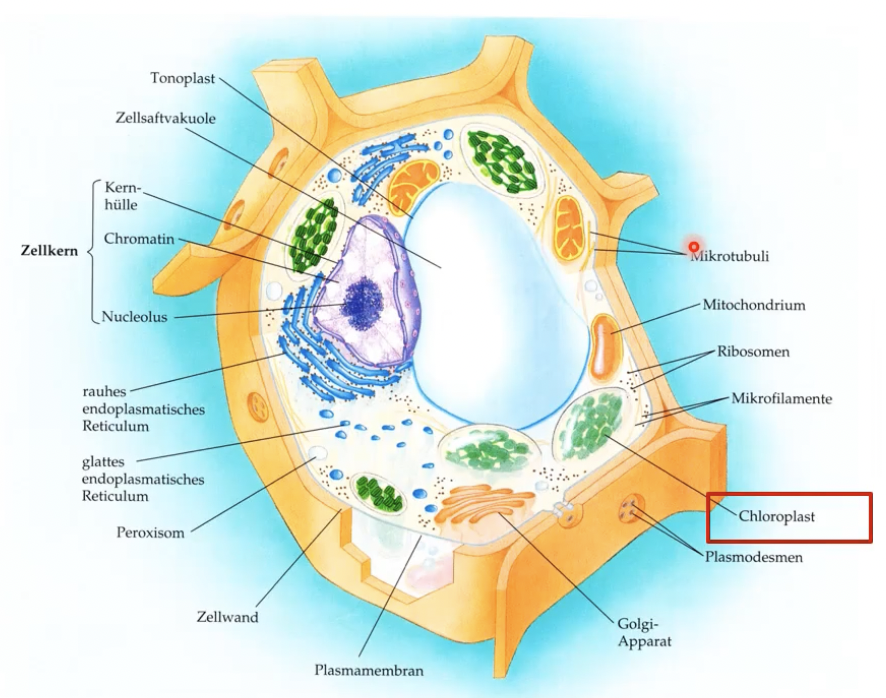
\includegraphics[width=10cm]{lec7/figures/pflanzenzelle.png}
\end{center}

\begin{itemize}
    \item \textbf{Zellkern} mit genetischem Material, Zusammenbau von Proteinen.
    \item \textbf{Mitochondrien} Energiebereitstellung, Kraftwerk der Zelle
    \item \textbf{Chloroplasten} Photosynthese \dangersign
\end{itemize}
(\dangersign \textit{Nenne drei Unterschiede zwischen einer pflanzlichen und tierischen Zelle})
\\\\
Bei der \textbf{Photosynthese} wird elektromagnetische Energie durch Chlorphylle absorbiert und in chemische Energie umgewandelt. Diese chem.\ Energie wird zum Aufbau von energiereichen chemischen organischen Verbindungen genutzt. In der \textbf{Lichtreaktion} \textcolor{red}{nehmen Pflanzen Licht und Wasser auf und erzeugen daraus NADPH, ATP und Sauerstoff} \dangersign. Im \textbf{Calvin-Zyklus} wird aus Kohlenstoffdioxid aus der Umgebung und den gebildeten NADPH \& ATP das Produkt Saccarose (Zucker) erzeugt. Der Wirkungsgrad beträgt dabei max. $E_{\text{chem}}/E_{\text{abs}}=20\%$ und die Effektivität (Nettoprimärproduktion) beträgt nur 0,8\% der Gesamteinstrahlung (großer Velust durch Reflektion). Durch die Primärproduktion werden ca. 100 Milliarden Tonnen Trockenmasse pro Jahr erzeugt, wobei marine Pflanzen nur marginal dazu beitragen. Wichtige Nebenprodukte sind Sauerstoff und fossile Energieträger.
\\\\
(\textit{Mögliche Klausurfrage: Nenne die Nettoreaktionsgleichung der Photosynthese.})

\begin{center}
    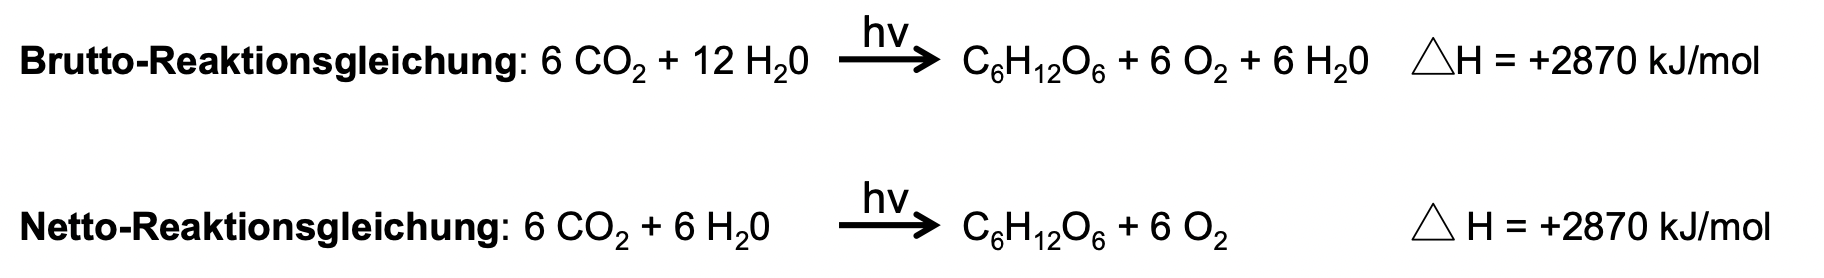
\includegraphics[width=14cm]{lec7/figures/gleichung.png}
\end{center}
\textbf{Inkohlung}: Pflanzen sterben ab, durch Sumpfgebiet wird aerobe Zersetzung verhindert und es bildet sich Torf. Sedimente lagern sich ab, hoher Druck presst Flüssigkeit aus dem Torf und es werden Brankohle, Steinkohle, Anthrazit gebildet.

\subsubsection{Sonnenkollektor}

Der Sonnenkollektor dient der Erwärmung von einfließendem kalten Wasser und ähnelt einem Wärmetauscher. Sonnenlicht fällt durch eine Glasplatte eine und das Wasserrohr absorbiert möglichst viel der einfalleden Strahlung. Der Betrieb des Sonnenkollektors erfordert das Pumpen des Wasserstroms durch den Kanal, wodurch die Effizienz des Systems reduziert wird. Wie kann der \textbf{Strömungswiderstand des Kanals optimiert} werden \dangersign?

\textit{Bionischer Prozess}: Studie über die \textbf{fraktale Kanalführung in Blättern} zur energieeffizienten Gestaltung von Kanalstrukturen für Solarabsorber. Die Strömungsbedingungen werden anhand des \textbf{Winkels der Verzweigungen} in der Kanalführung optimiert. Das Optimum befindet sich bei Winkeln von 145° (auch bei Blättern vorzufinden). Dadurch kann der erforderliche Druck und die daran gekoppelte notwendige Pumpleistung verringert werden. Aus diesem Ansatz hat sich ein \textbf{bionisches Produkt, die Software Fractherm} entwickelt, welche fraktale Kanalstrukturen für Solarabsorber modelliert \dangersign.

\begin{center}
    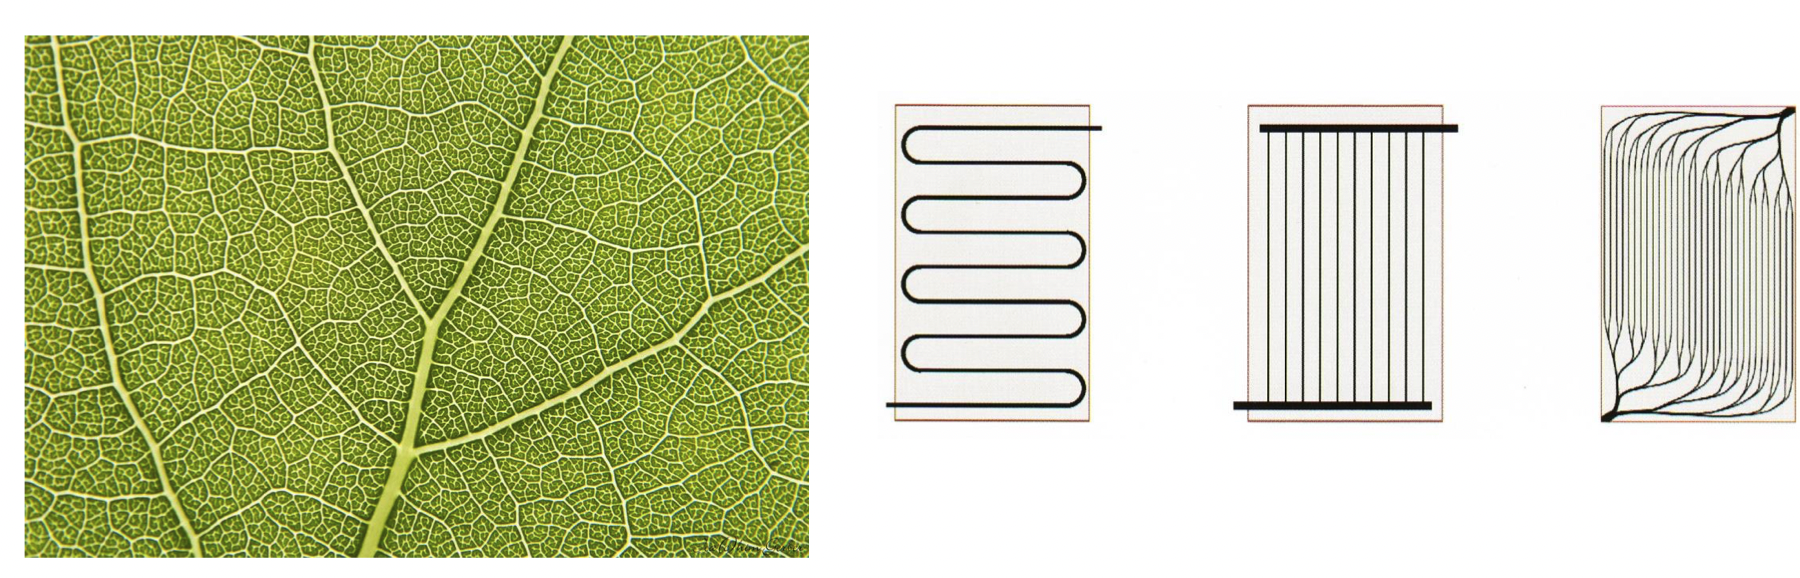
\includegraphics[width=12cm]{lec7/figures/kanal.png}
    \hfill
    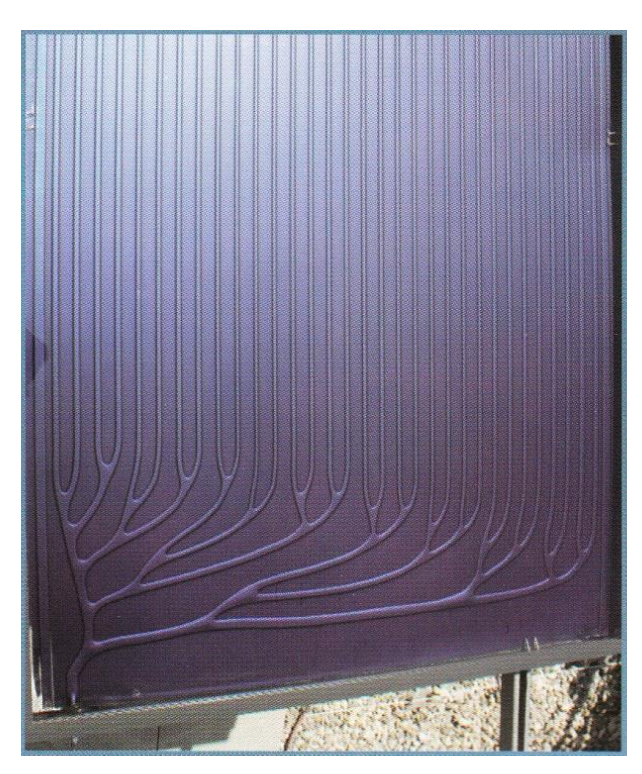
\includegraphics[width=4cm]{lec7/figures/fraktal.png}
\end{center}
Prinzipiell lässt sich Sonnenenergie durch Sonnenkollektoren (Warmwassererzeuger/Solarthermie), Sonnenwärmekraftwerke, Solarkocher und indirekt durch Winkraft und Biokraftstoffe nutzen.
\\\\
Vorteile von alternativen Energien ggü.\ fossilen Energieträgern:

\begin{itemize}
    \item (Praktisch) unbegrenzte Verfügbarkeit
    \item Klimaschonend ($CO_2$)
    \item Keine Feinstaubbelastung
    \item Geringe Abhängigkeit von Ölstaaten
\end{itemize}
Nachteile:
\begin{itemize}
    \item Fluktuation (Wetter-/ Jahreszeitabhängig)
    \item Energieintensive Produktion
    \item Speicherkapazitäten und Netzwerk
\end{itemize}
Der Wirkungsgrad von Solarzellen außerhalb von Laborbedingungen bis zu 17\% und ist damit vergleichbar mit der Photosynthese ($\rightarrow$ wurde nicht weiter vorgestellt, da es nicht wirklich bionisch ist).
\\\\
\textit{Bionische Anwendung von einem selbstausrichtendem Sonnekollektor:} Sonnenkollektoren müssen mit Motorkraft dem Sonnenstand nachgeführt werden. Dieses Nachführen wird vermieden, indem man den Kollektor als innenverspiegelten, parabolischen Trichter ausführt. Dabei dient die Wüstenpflanze Fenestraria als biologisches Vorbild, bei der das eintreffende Licht durch Wasserzellenstruktur aus jeder Einfallsrichtung auf die fotosynthetischen Zellen gestreut wird.
\begin{center}
    \includegraphics[width=6cm]{lec7/figures/wüstenpflanze.png}
\end{center}

\subsubsection{Solarbetriebene Hornissen}

Die Wechselwarmen Insekten haben eine geringe Aktivität bei kühlen Temperaturen, sodass Aufwärmphasen eine Gefahr durch Prädatoren darstellen. Bei der Orientalischen Hornisse weisen die braunen Streifen Kerben auf, die Reflexionen verringern und die gelben Strreifen wandeln das Sonnenlicht in elektrische Energie durch das Pigment Xanthopterin um.

\subsubsection{Schmetterlingsflügel als Solarfänger}

Schmetterlinge verfügen über feinstrukturierte Schuppen auf den Flügeln (siehe die nachfolgende Abbildung). \textbf{Wozu dient diese Feinstrukturierung \dangersign?}
\begin{itemize}
    \item Erhöhen durch veränderte Fluidreibung den aerodynamischen Auftrieb um ca.\ 10\%
    \item Erzeugen Schillerfarben durch Interferenz (Strukturfarben $\rightarrow$ kein Pigment!). 
    \item Thermoregulation (optimale Betriebstemperatur 40° im Thorax)
    \begin{itemize}
        \item Nutzen Flügelstellung zur Reflexion der Strahlen auf den Thorax
        \item Thoraxschuppen verhindern Wärmeverlust
        \item Flügeladern sind mit Hämolymphe durchströmt und leiten Wärme in den Thorax
    \end{itemize}
\end{itemize}
Auf der rechten Seite der folgenden Abbildung ist der Reflexionsgrad des einfallenden Lichtes über den Wellenlängenbereich des sichtbaren Lichts eingezeichnet. Der schwarze Schmetterling absorbiert fast das gesamte Licht, während der weiße Schmetterling einen Großteil reflektiert. Ein entschuppter Flügel reflektiert fast kein Licht mehr.

\begin{center}
    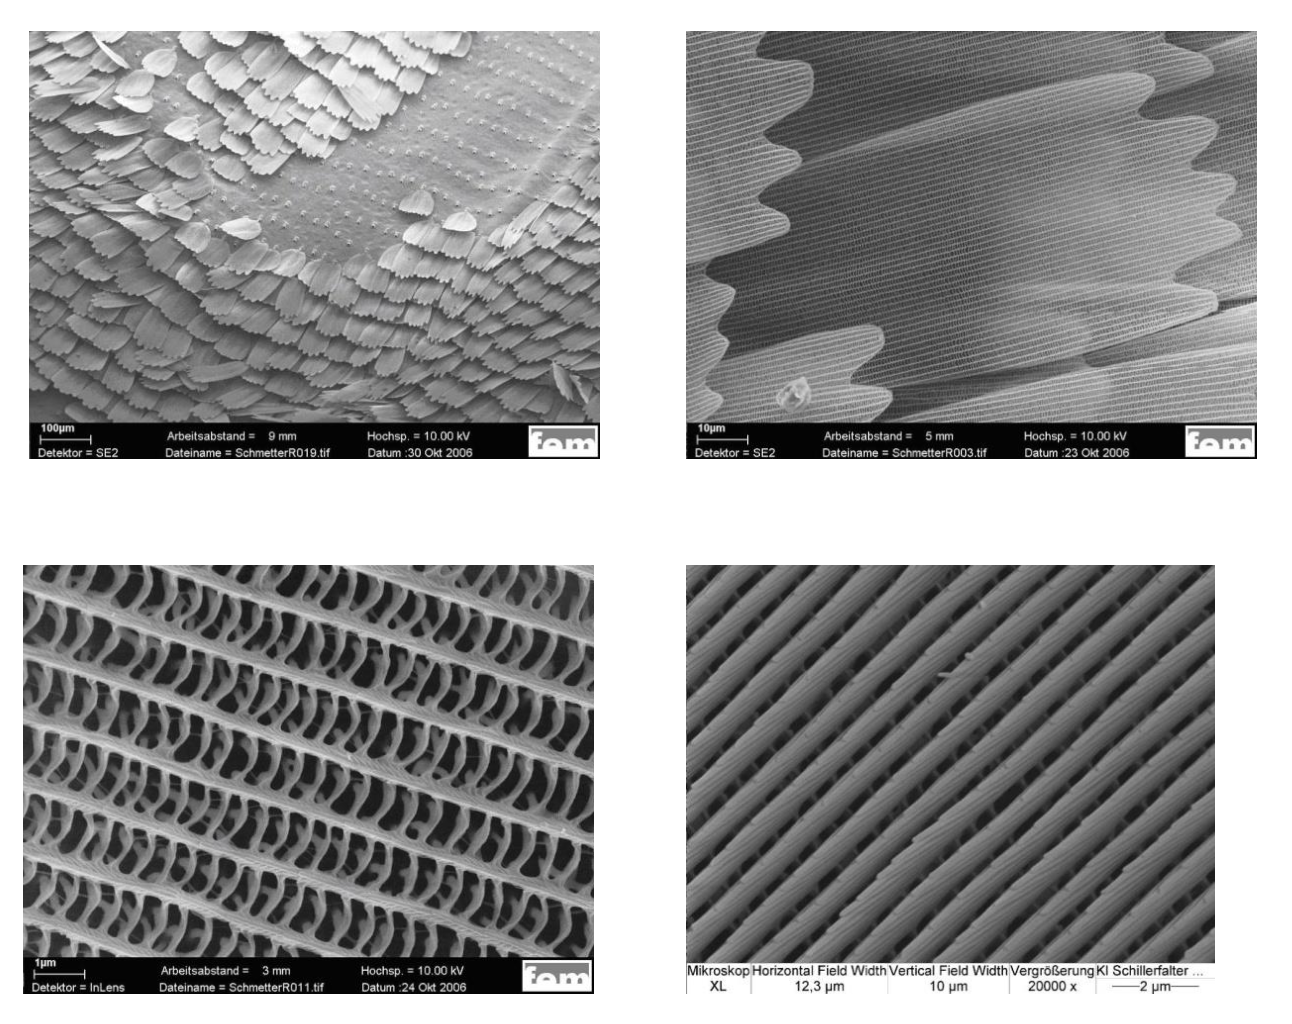
\includegraphics[width=8cm]{lec7/figures/schmetterling.png}
    \hfill
    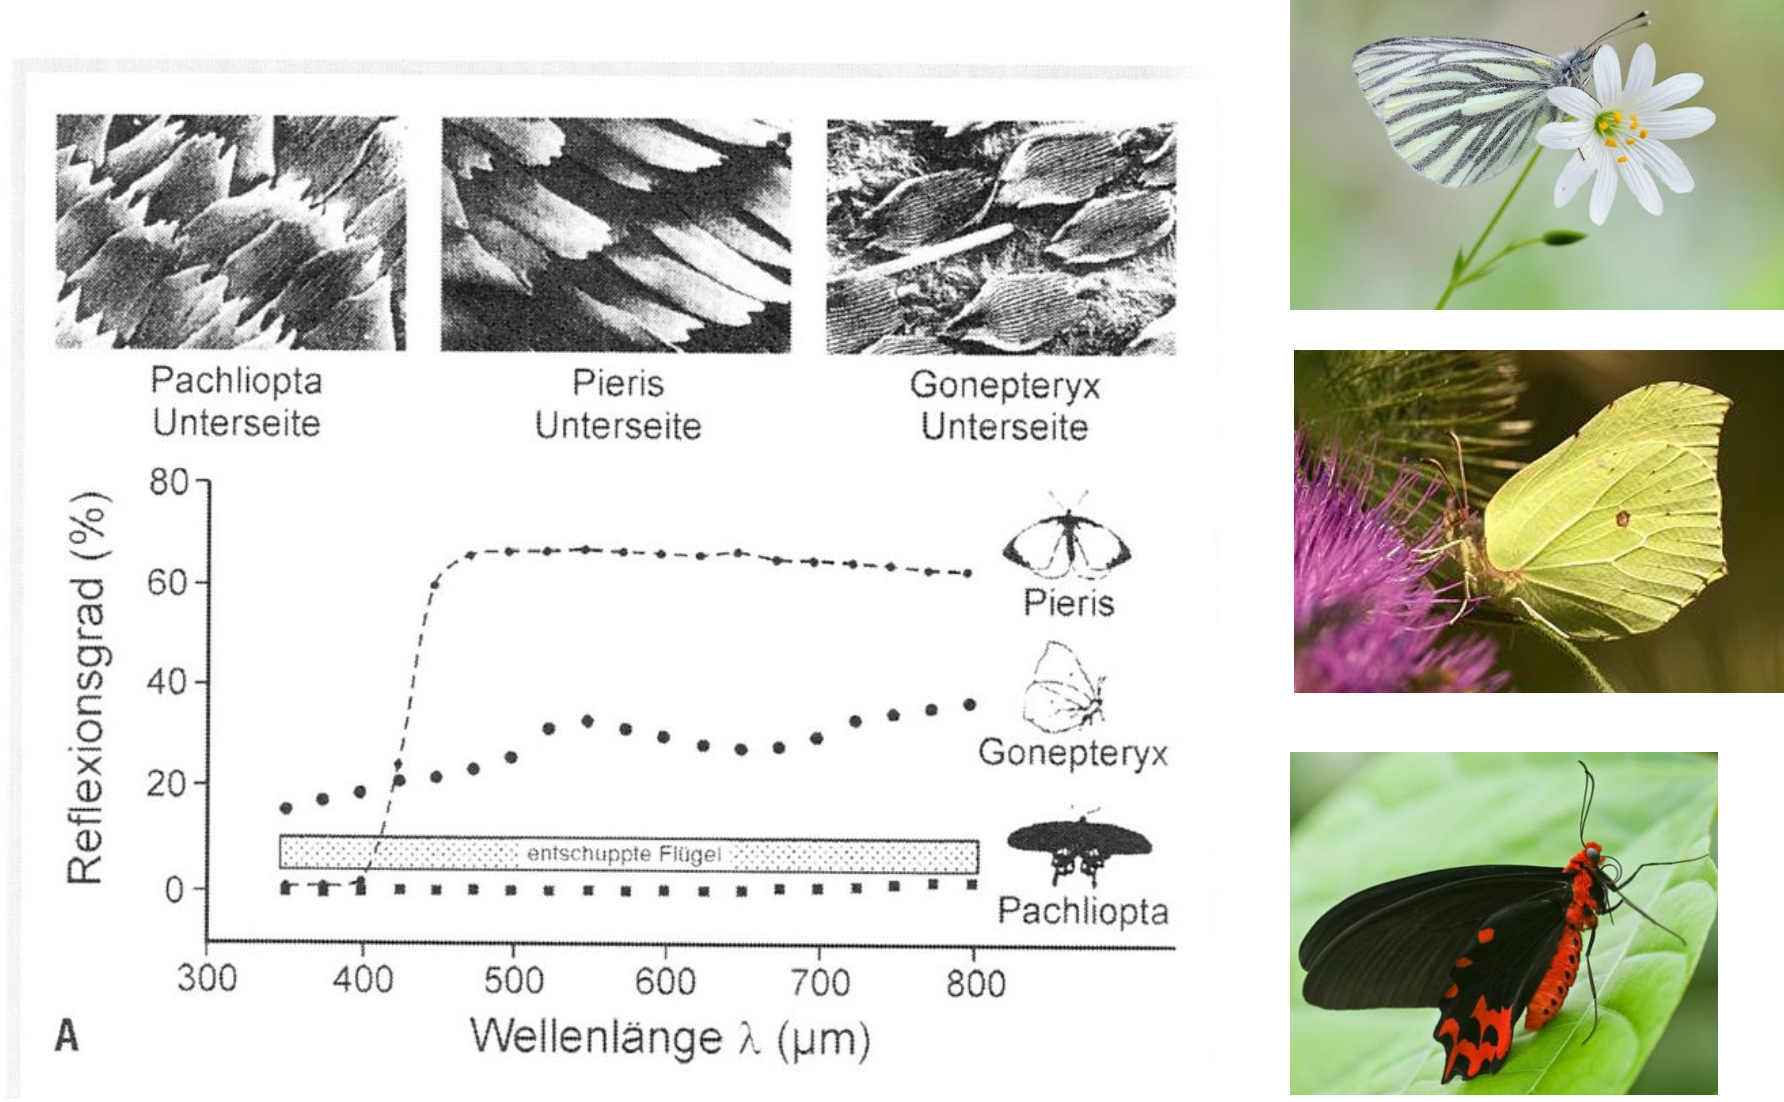
\includegraphics[width=8cm]{lec7/figures/absorption.png}
\end{center}
\textit{Bionische Anwendung:} Gerade Spezialisten sind hierfür besonders interessant -- der Alpenapollo kommt in Höhen bis 2800m vor. Es könnte gezeigt werden, dass die Schuppen den wesentlichen Beitrag zur Absorption des Sonnenlichtes stellen und der Schmetterling dadurch in der Lage ist, seinen Thorax auf bis zu 59°C aufzuwärmen (vgl.\ mit 11°C beim entschuppten Flügel). Es wird vermutet, dass der Abstand zwischen den Längsrippen auf den Schuppen ja nach Verhältnis zur Wellenlänger des einfallenden Lichts zu Reflektion ($\rightarrow$ Kühlung von z.B.\ Mikrochips) oder zu Interferenz ($\rightarrow$ Aufheizen, z.B.\ Verbesserung von Solarzellen) führen.

\subsection{Baubionik}

\subsubsection{Bio-/Natur-inspiriertes Bauen} 

Der Münchner Architekt Frei Otto entwarf die frei hängenden Dächer des Olympiastations in München nach dem Vorbild von ``hängender'' Seifenhaut. Im Stuttgarter Flughafen wurden Trägerstrukturen von Bäumen abstrahiert.

\begin{center}
    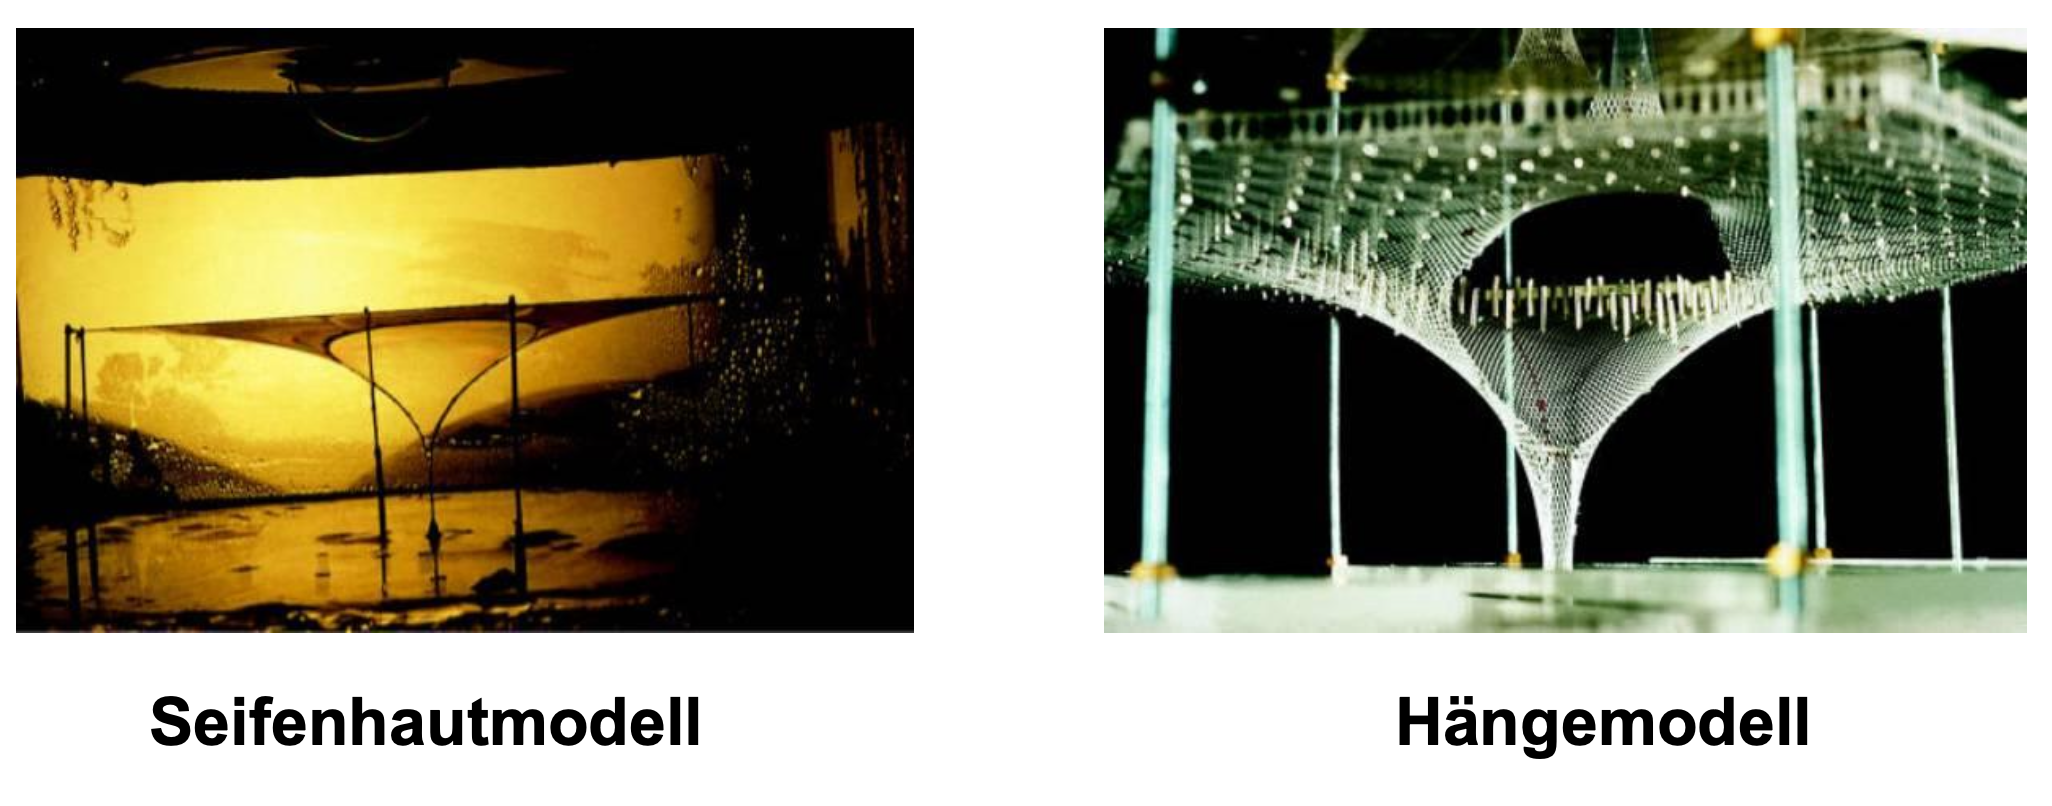
\includegraphics[width=8cm]{lec7/figures/seife.png}
    \hfill
    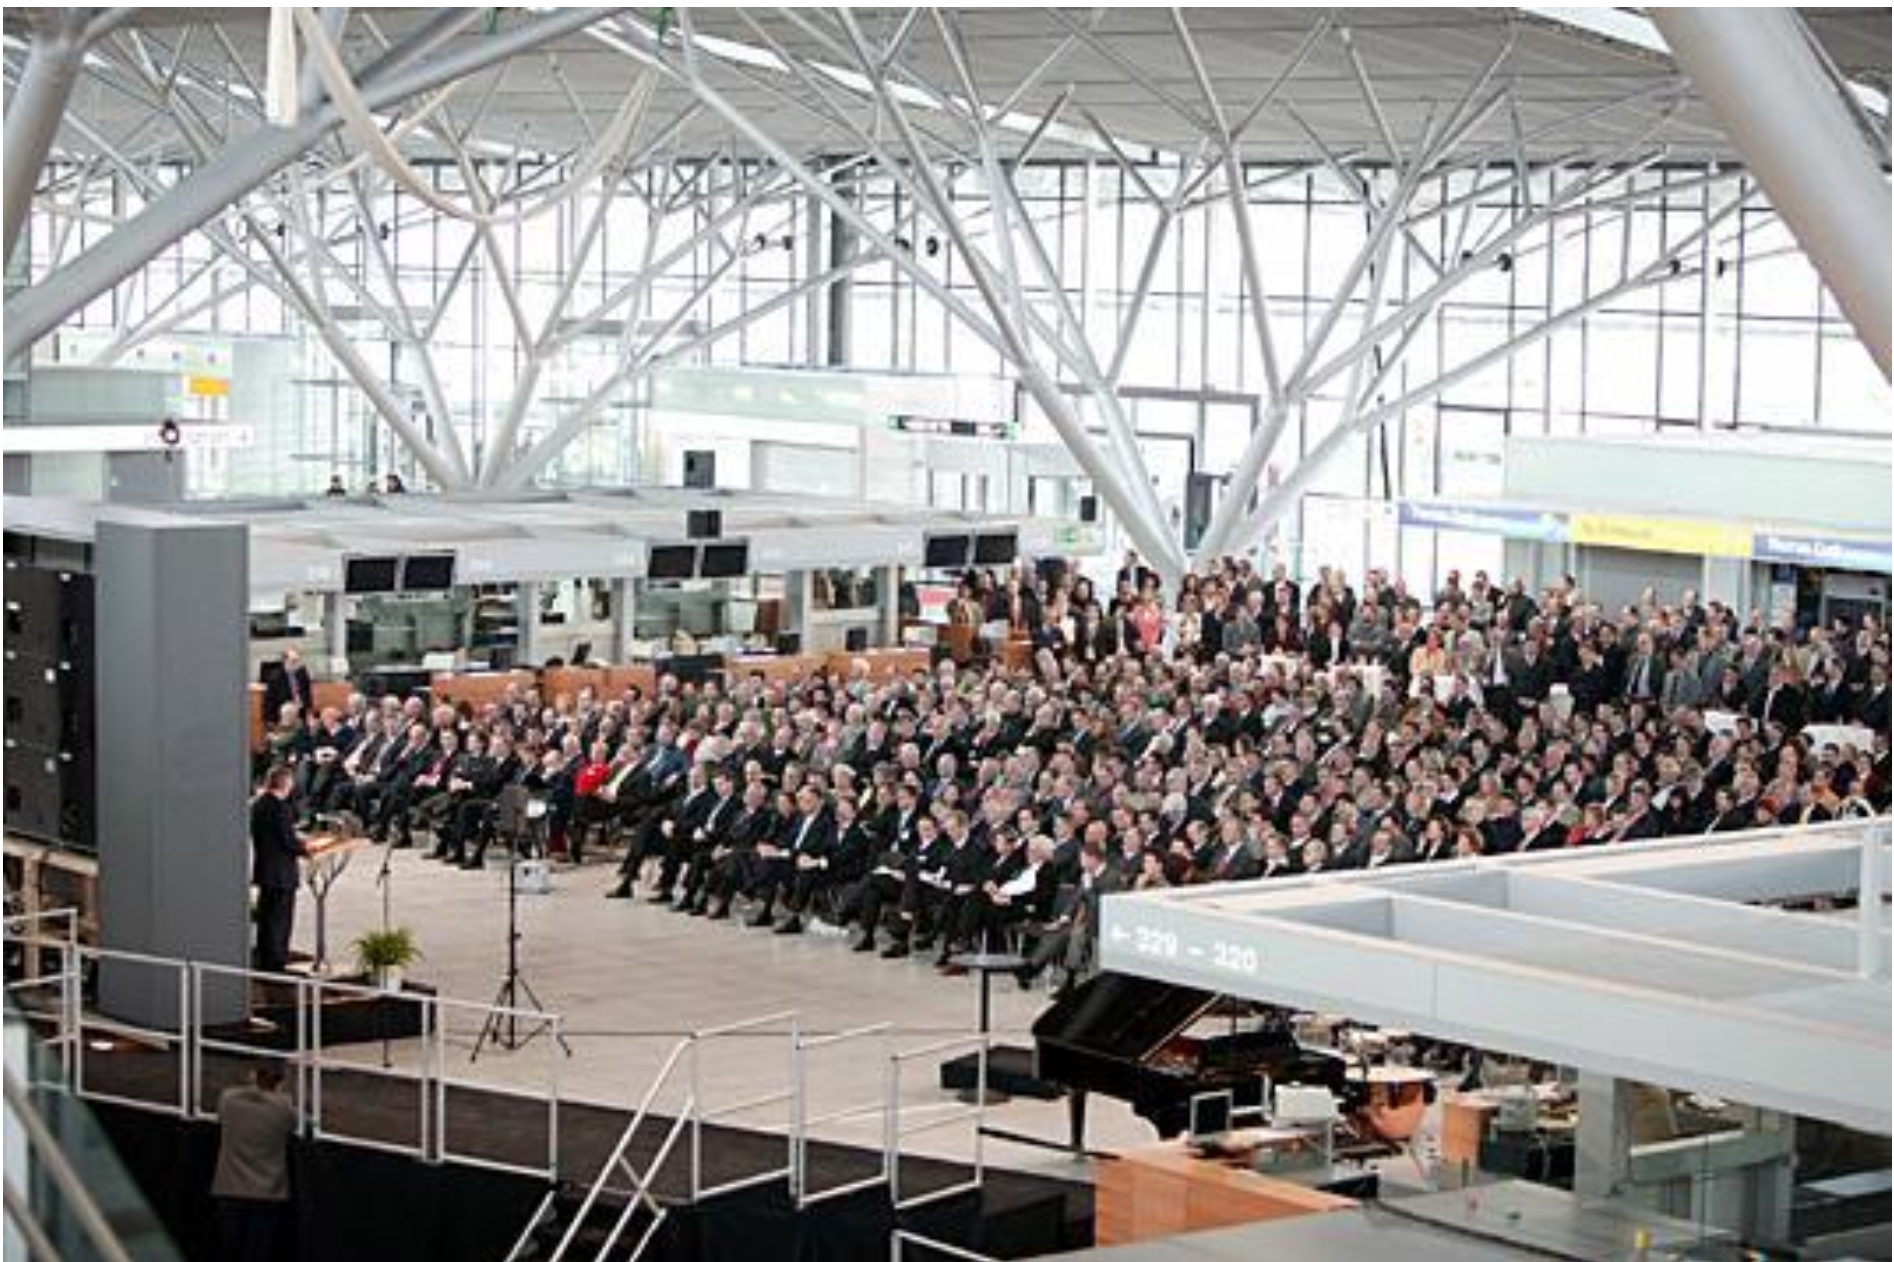
\includegraphics[width=6cm]{lec7/figures/flughafen.png}
\end{center}
Gerade die biologischen und technischen Materialien unterscheiden sich wesentlich:

\begin{center}
    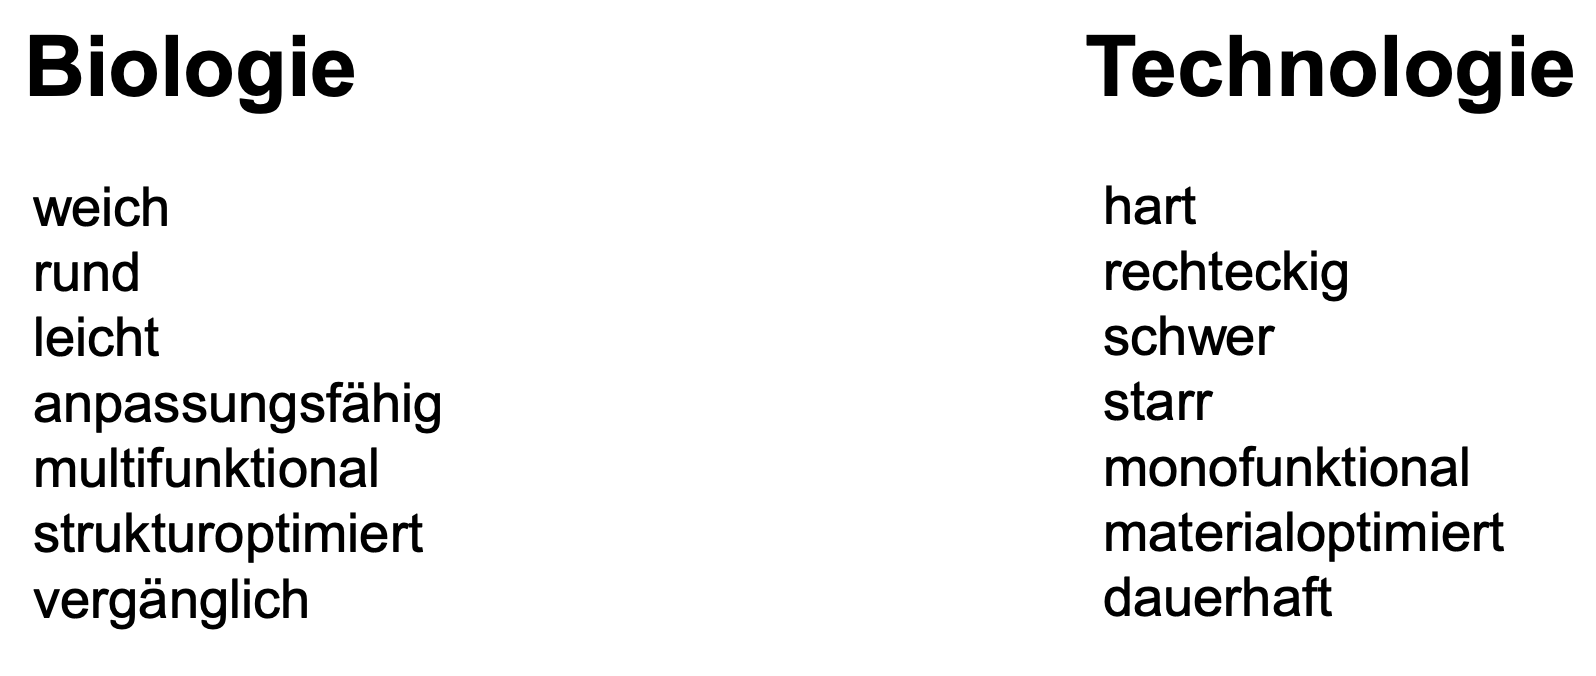
\includegraphics[width=8cm]{lec7/figures/material.png}
\end{center}
Der die Glasstruktur des Kristallpalasts in London wurde nach dem Vorbild der Seerose Gebaut. Der geodäsische Pavillon von Buckminster Fuller ist am Silicatskelett der Radiolarie (ein einzelliger Organismus) inspiriert. Gerade die Strukturen von Radularien können bei vielen technischen Anwendungen genutzt werden, um eine optimale Balance aus Gewichtsersparnis, Fertigungsaufwand und Herstellungskosten zu erreichen.

\begin{center}
    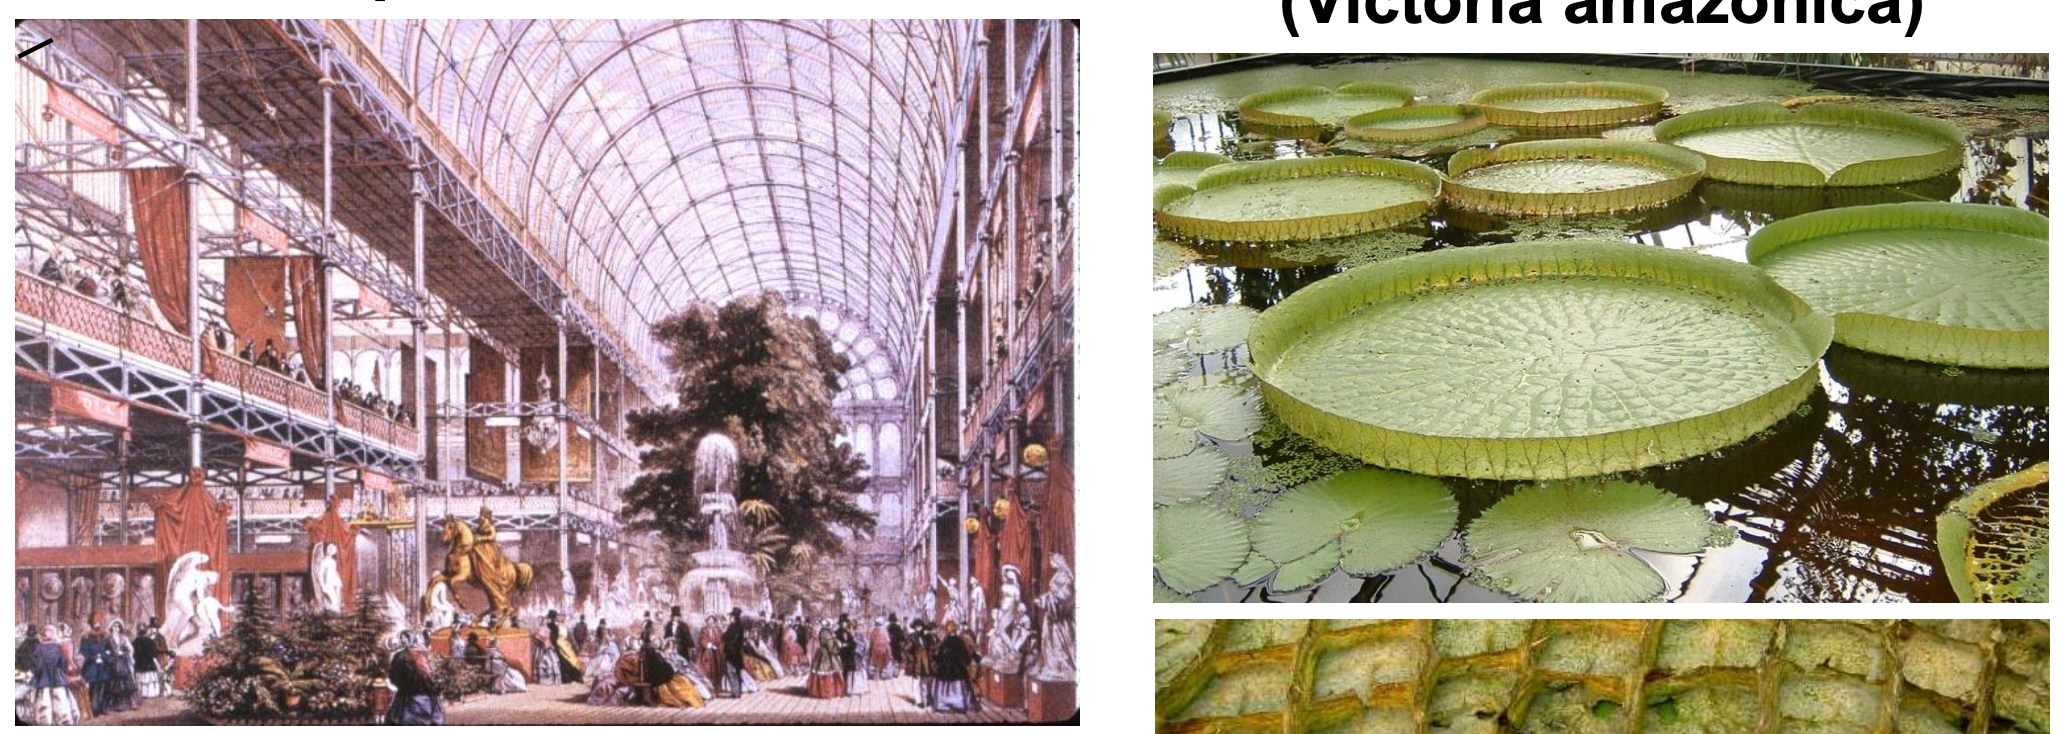
\includegraphics[width=8cm]{lec7/figures/palast.png}
    \hfill
    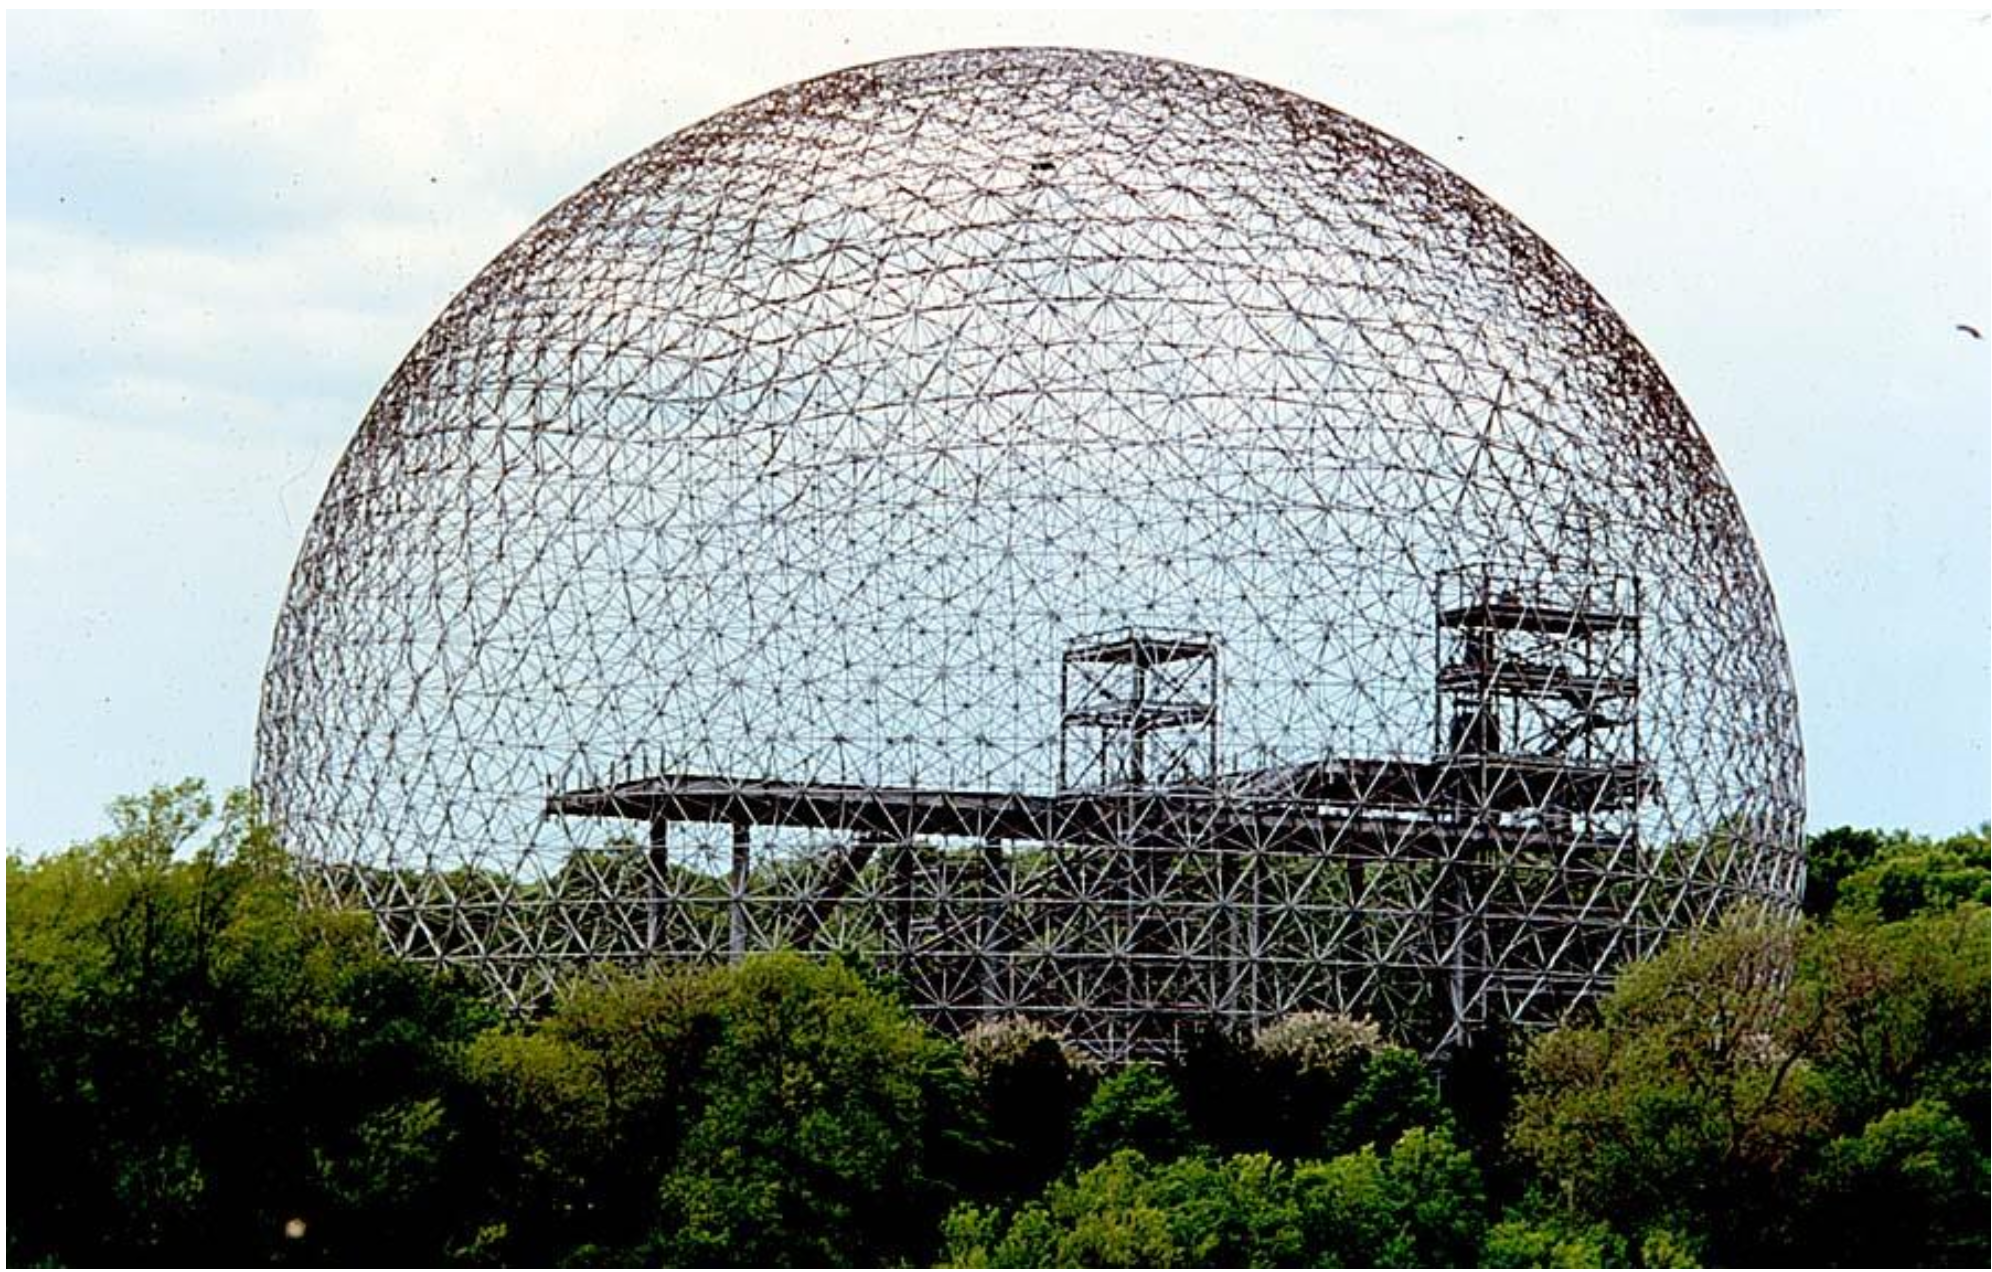
\includegraphics[width=4cm]{lec7/figures/pavillon.png}
    \hfill
    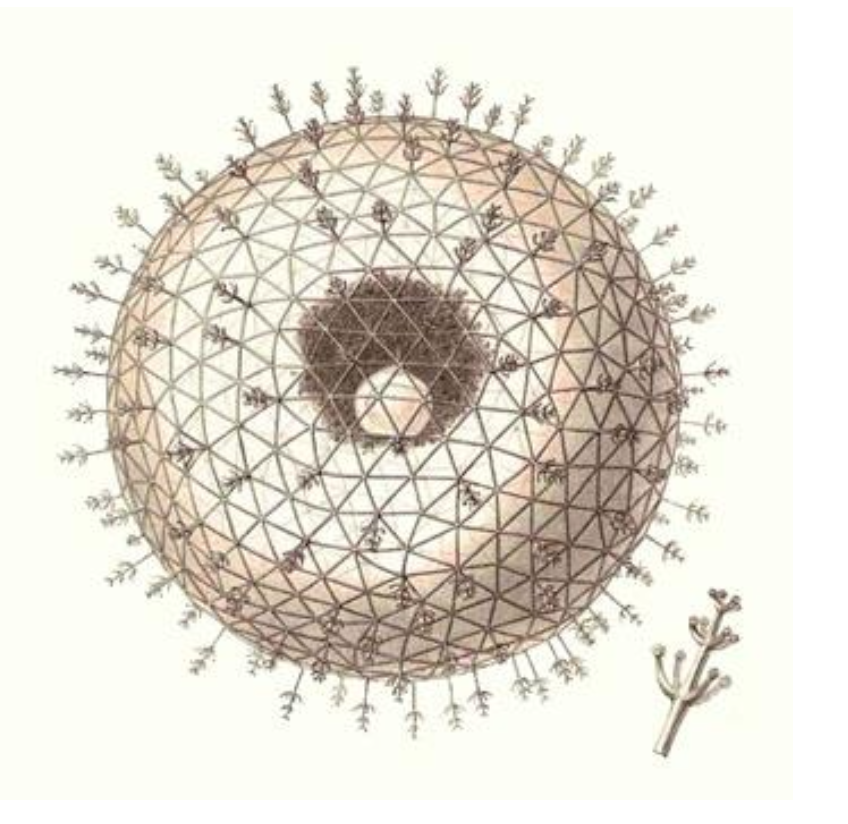
\includegraphics[width=3cm]{lec7/figures/radularie.png}
\end{center}

\paragraph{Methode der Zugdreicke \dangersign} Stämme brechen selten, was an der Ausprägung der Kerben bei Verzweigungen liegt. Bei der Methode der Zugdreicke entsteht die Materialoberfläche indem man zwei Schnittpunkte von einem Kreis und der bisherigen Oberfläche findet, diese verbindet und anschließend das Vorgehend iterativ von dem Mittelpunkt der Verbindungslinie weiterführt. Es zeigt sich, dass bei einer solchen Kerbe die Spitzenbelastung geringer als bei einer Ingenieurskerbe ist.
\\\\
\textit{Bionische Anwendung:} Um die Kerben in den Gewinden von orthopädischen Schrauben so zu gestalten, dass Spannungsspitzen in der Belastung vermieden werden $\rightarrow$ mehr Lastwechsel bis zum Auftreten von Rissen möglich.

\begin{center}
    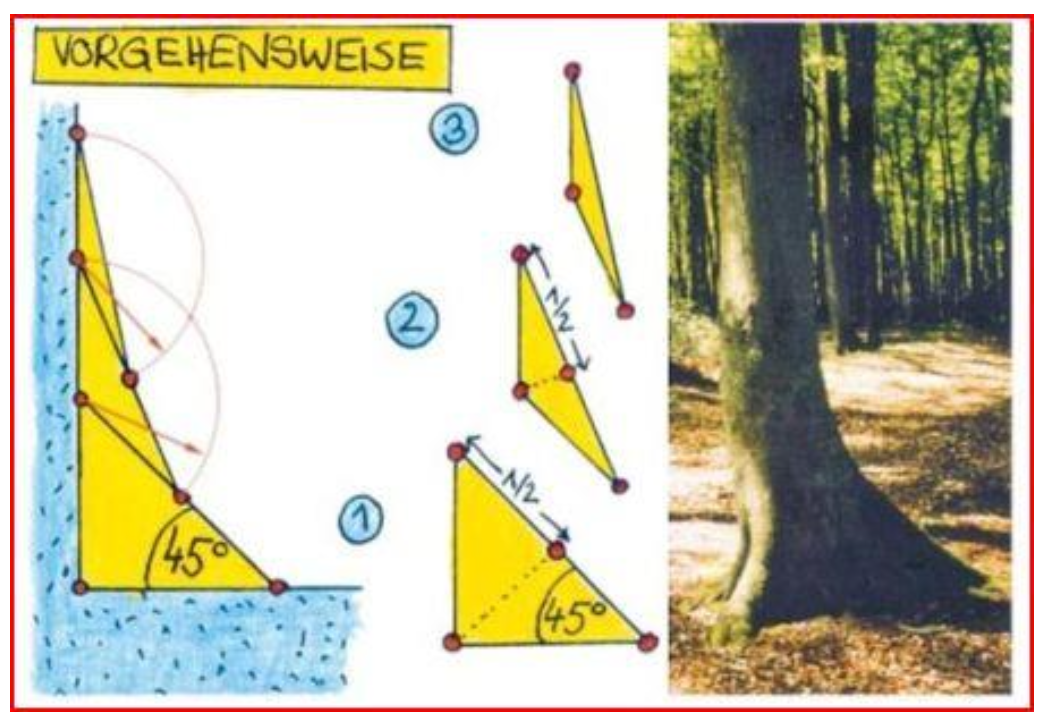
\includegraphics[width=6cm]{lec7/figures/zugdreiecke.png}
    \hfill
    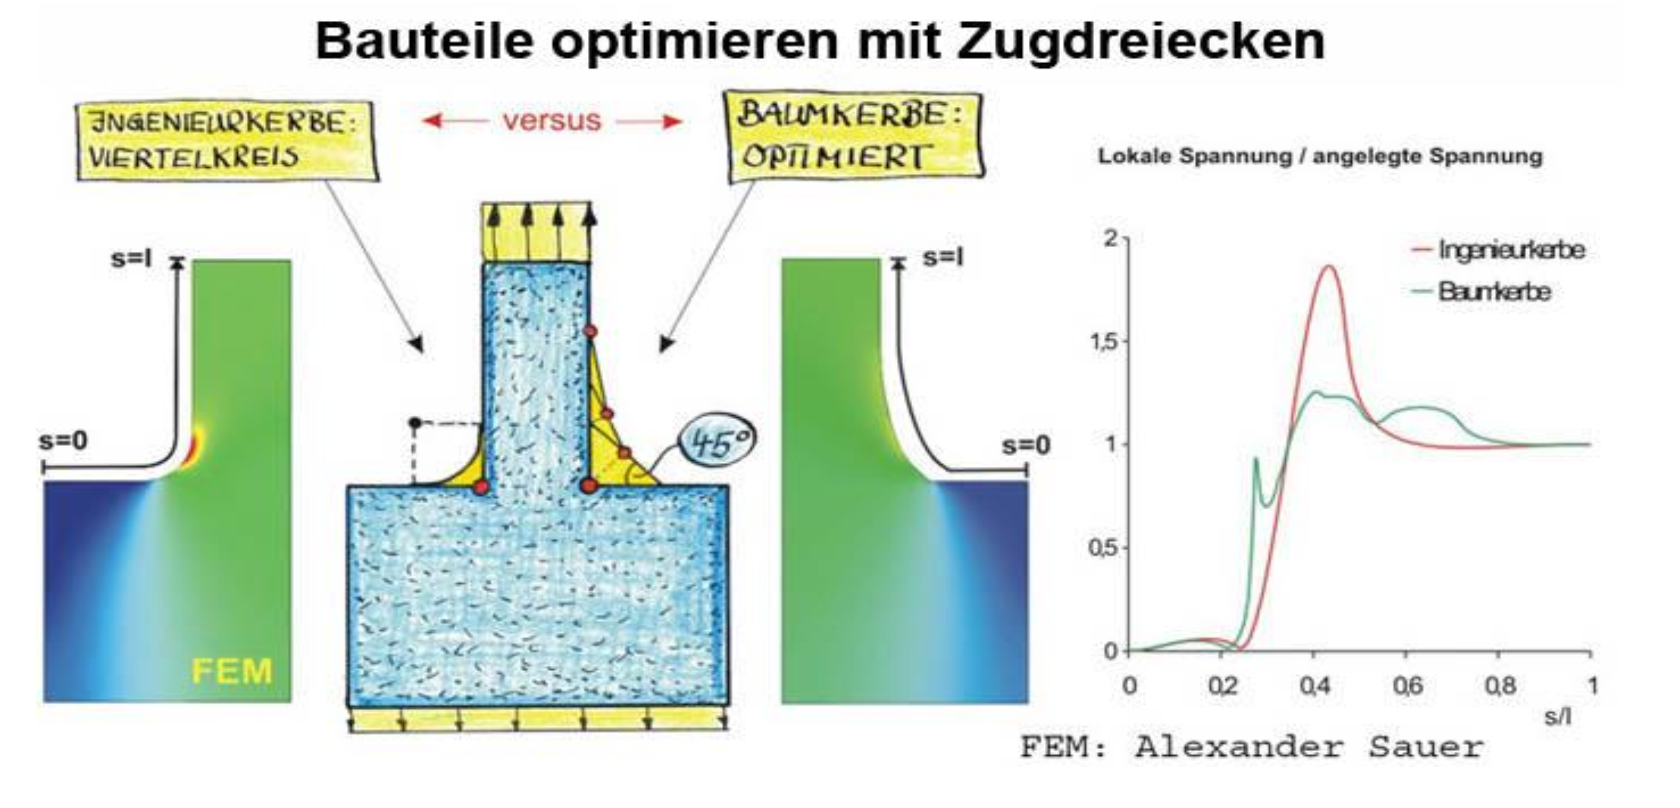
\includegraphics[width=8cm]{lec7/figures/kerbe.png}
\end{center}
\textbf{Kakteen} verwenden \textit{nicht die Methode der Zugdreiecke}, da sie als Einkeimblättrige Pflanzen kein Holz bilden.
Stattdessen haben sie ein Festigungsgewebe mit Holzlamellen zur Stabilisierung. Dieses Gewebe kann technisch mit einem speziellen 3D Flechtverfahren abstrahiert werden, um ein Seil mit Verzweigungen zu erzeugen, welches an der Verzweichung keine Schwachstelle aufweist.
\\\\
(\dangersign \textit{Skizziere eine Baumverzweigung. Welche Pflanze macht das anders? Was ist die bionische Umsetzung?})

\subsubsection{Baubotanik}

In Asien werden Gerüste für Fassadenarbeiten vorwiegend aus Bambus gebaut. Auch in Europa gibt es Projekte, bei denen Objekte, z.B.\ ein Metallsteg, ohne Schrauben/Nägeln an Bäumen befestigt wird und durch deren Wachstum stabilisiert wird.

\begin{center}
    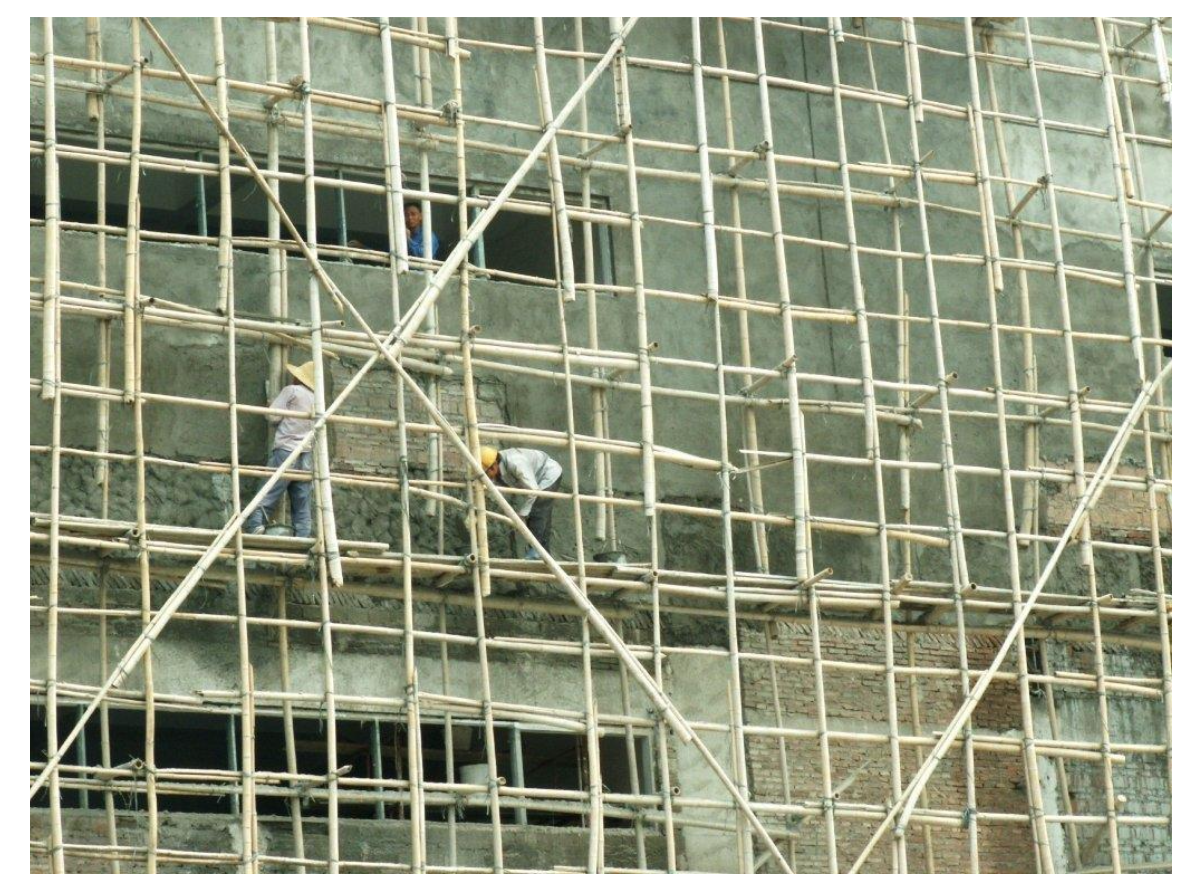
\includegraphics[width=5cm]{lec7/figures/bambus.png}
    \hfill
    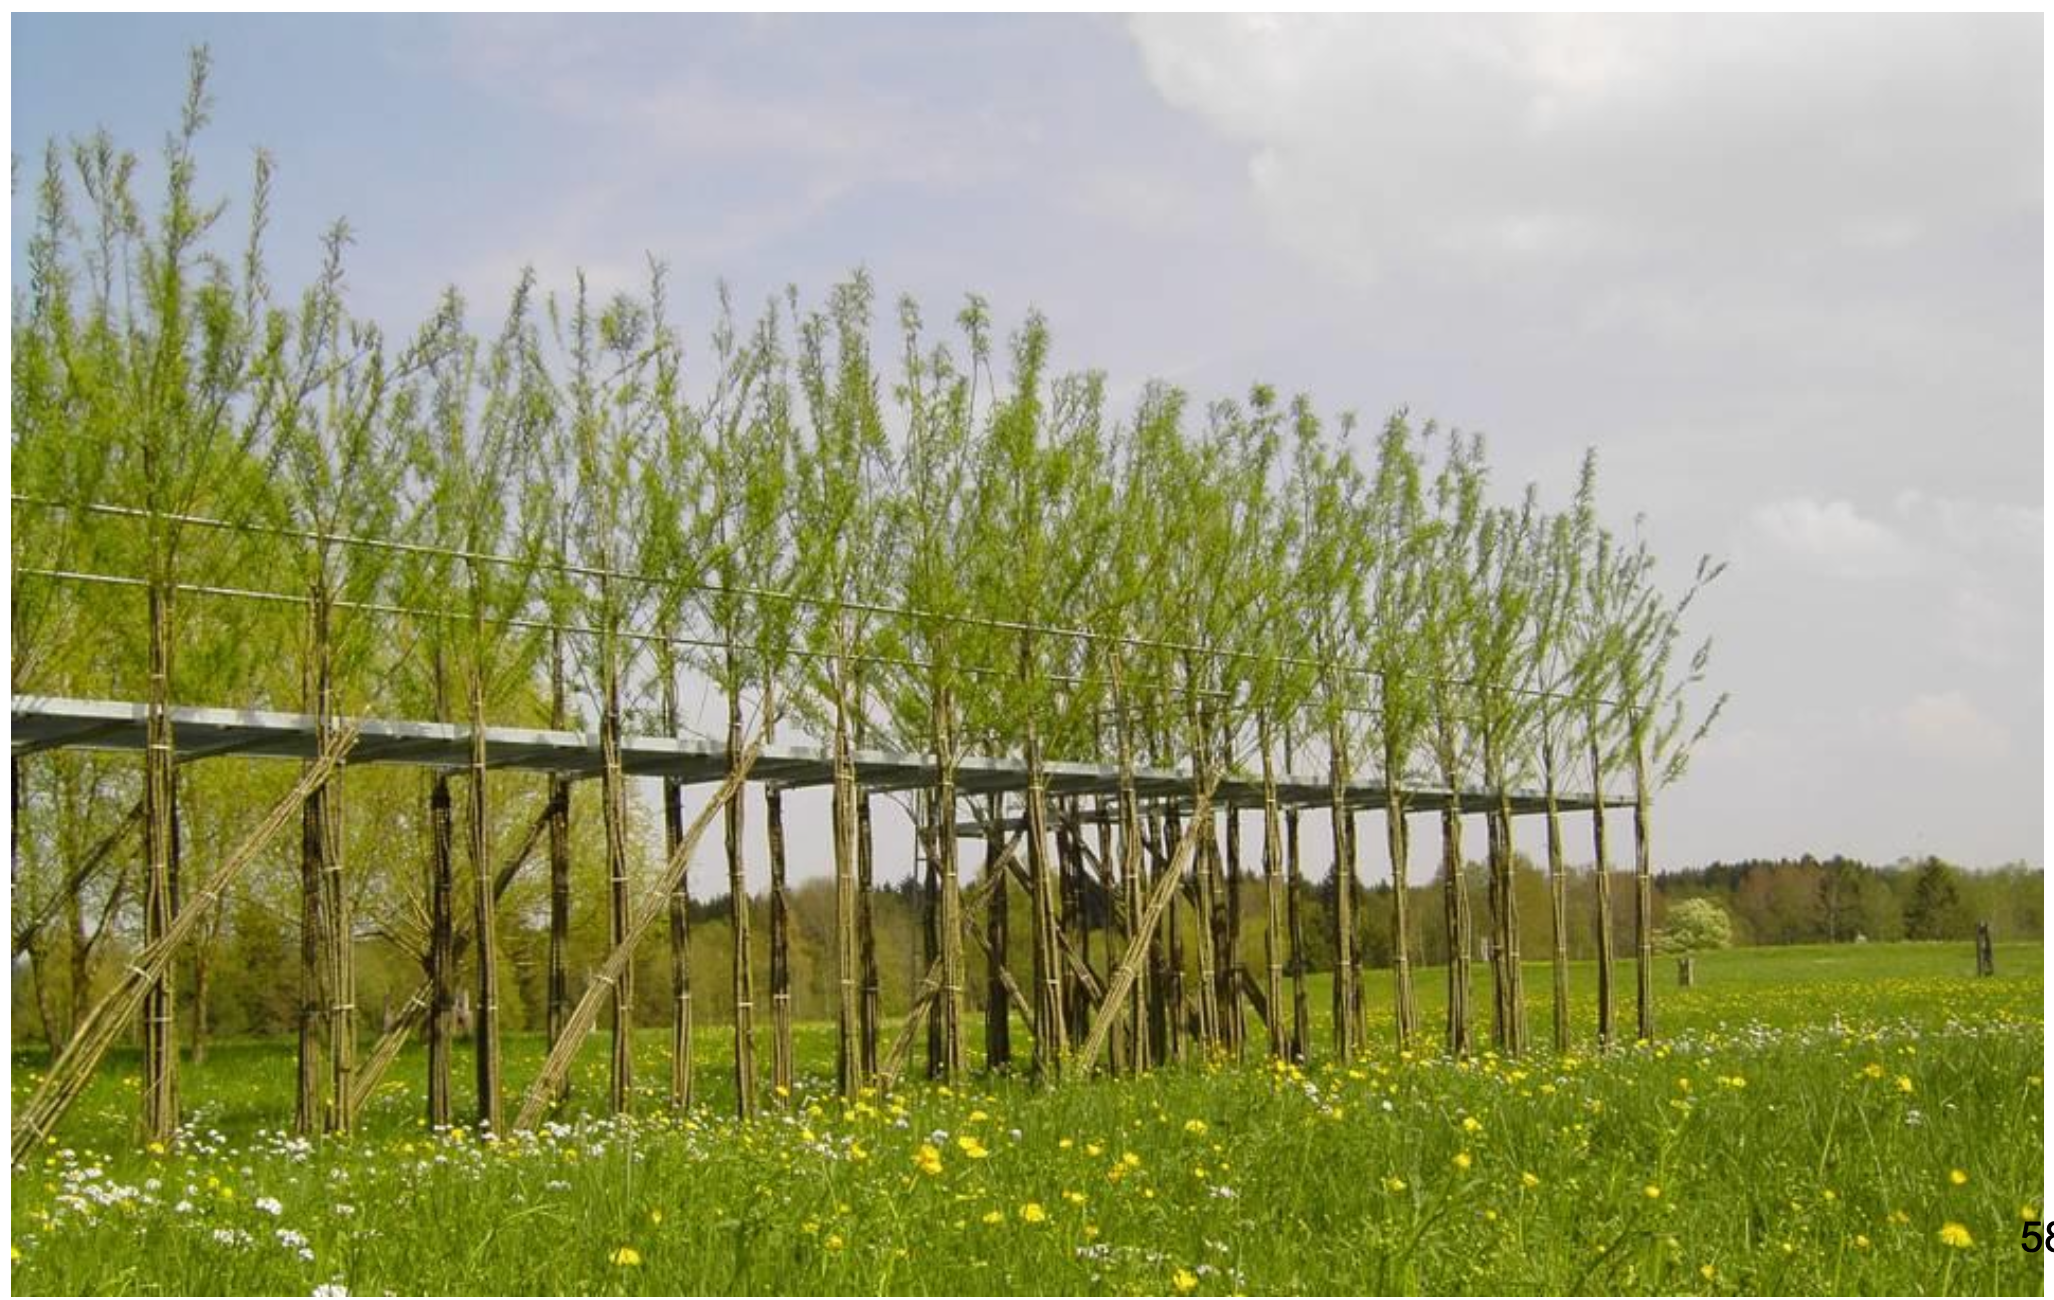
\includegraphics[width=5cm]{lec7/figures/steg1.png}
    \hfill
    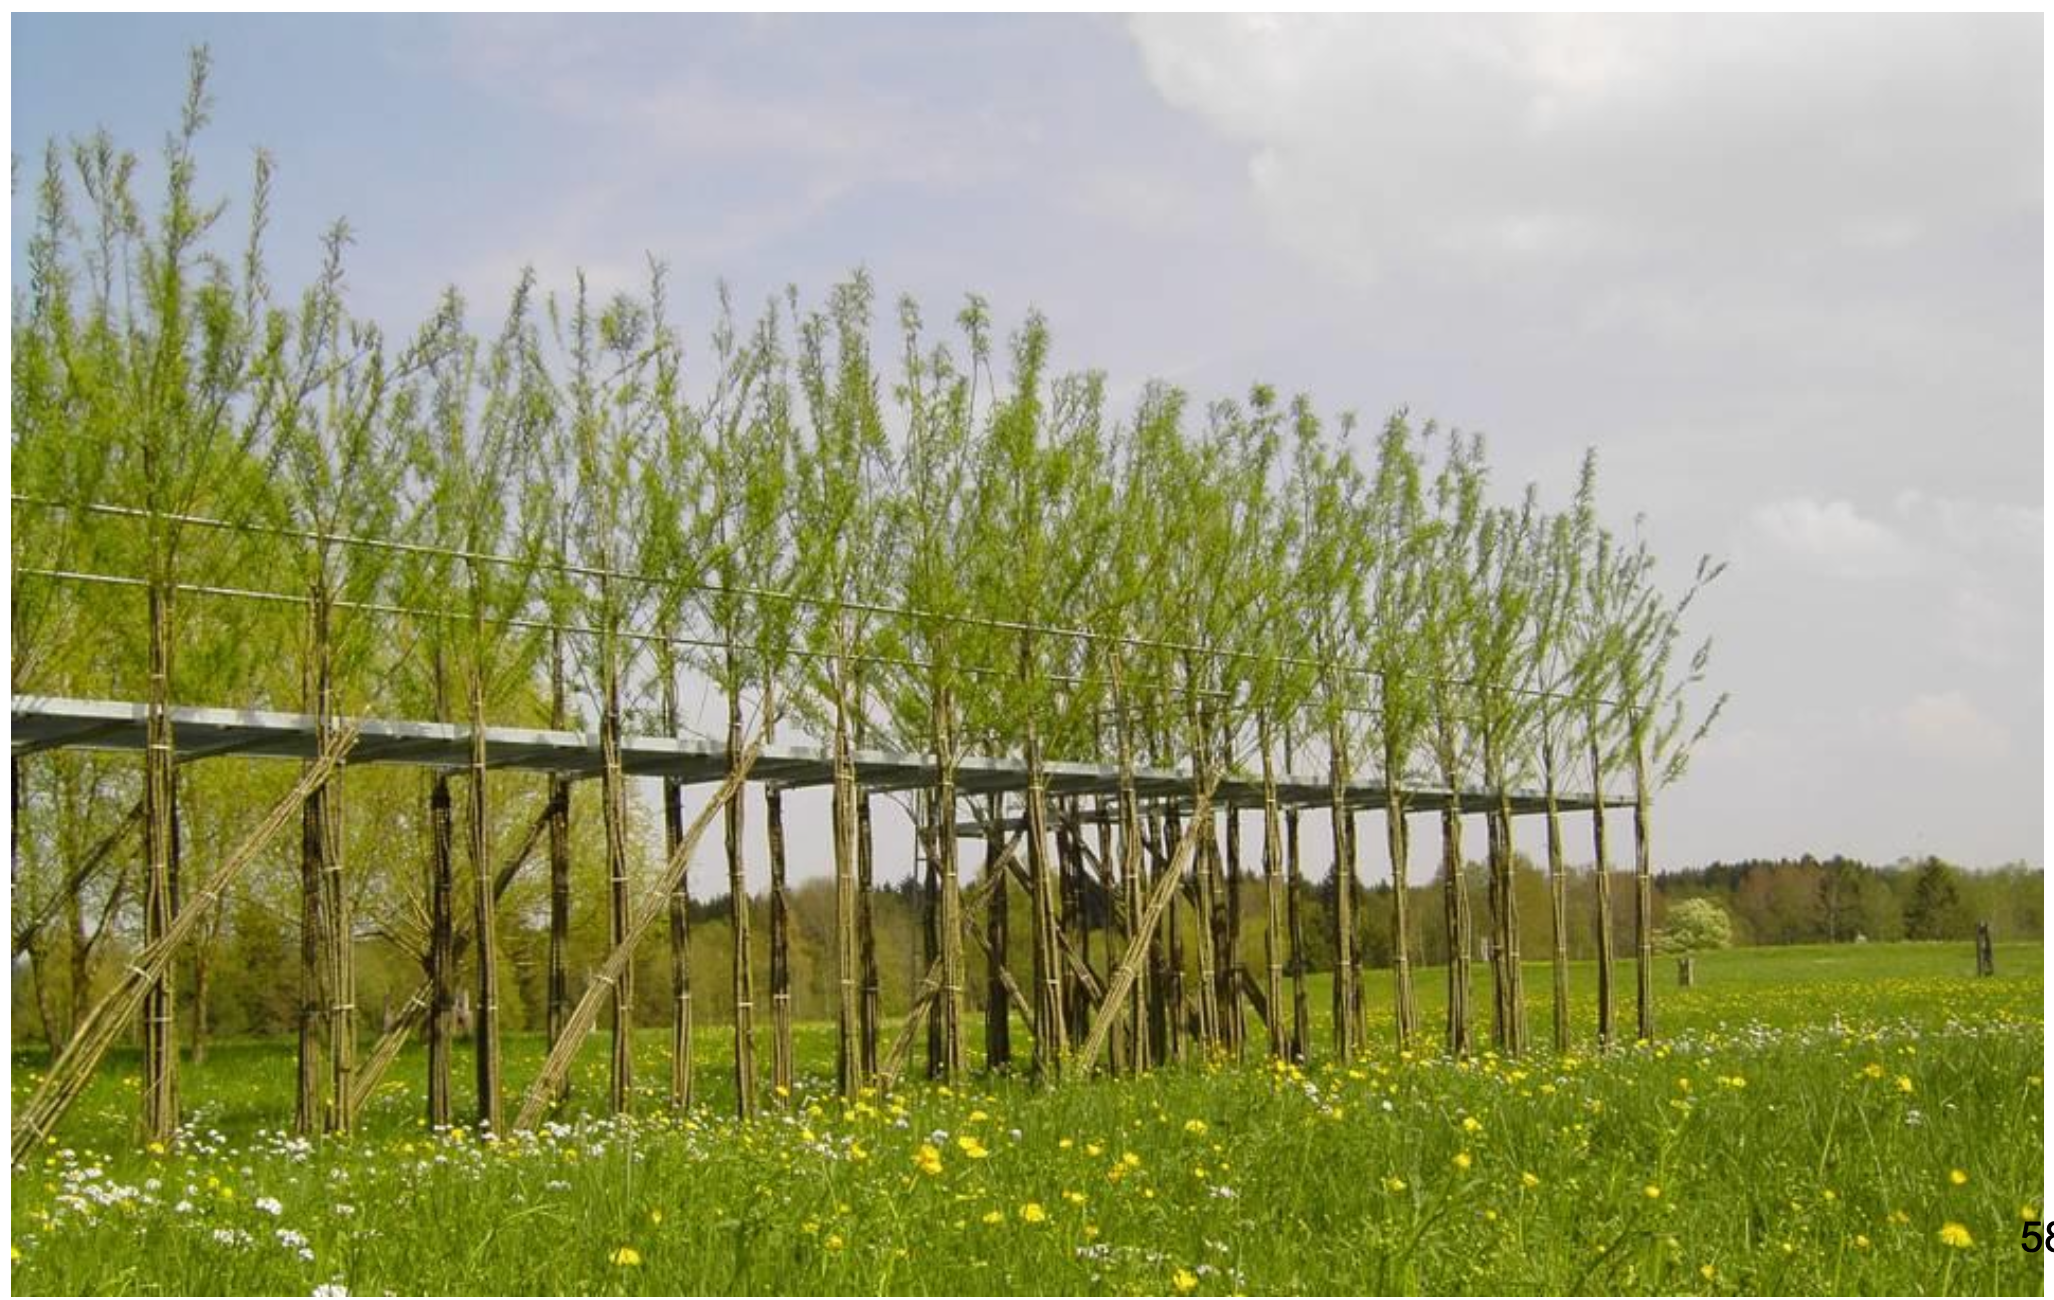
\includegraphics[width=5cm]{lec7/figures/steg1.png}
\end{center}

\subsubsection{Wandelbarer Leichtbau in der Architektur}

Es gibt unterschiedliche Pflanzenbewegungen in der Natur. Diese können autonom entstehen, wobei Aktive Bewegungen auf die Umgebung reagieren, oder müssen von außerhalb aktiviert werden (nicht-autonom). Lose aufgehängte Pflanzenorgane werden bspw.\ vom Wind gelöst und fortgetragen, während diese bei elastischer Deformation durch Belastung gewisser Druckpunkte (z.B.\ durch mechanische Interaktionen mit einem Bestäuber) die Bewegung auslösen. Diese Bewegung kann (z.B.\ bei Blüten), aber muss nicht (z.B.\ für den Abwurf von Samen) reversibel sein.

\begin{center}
    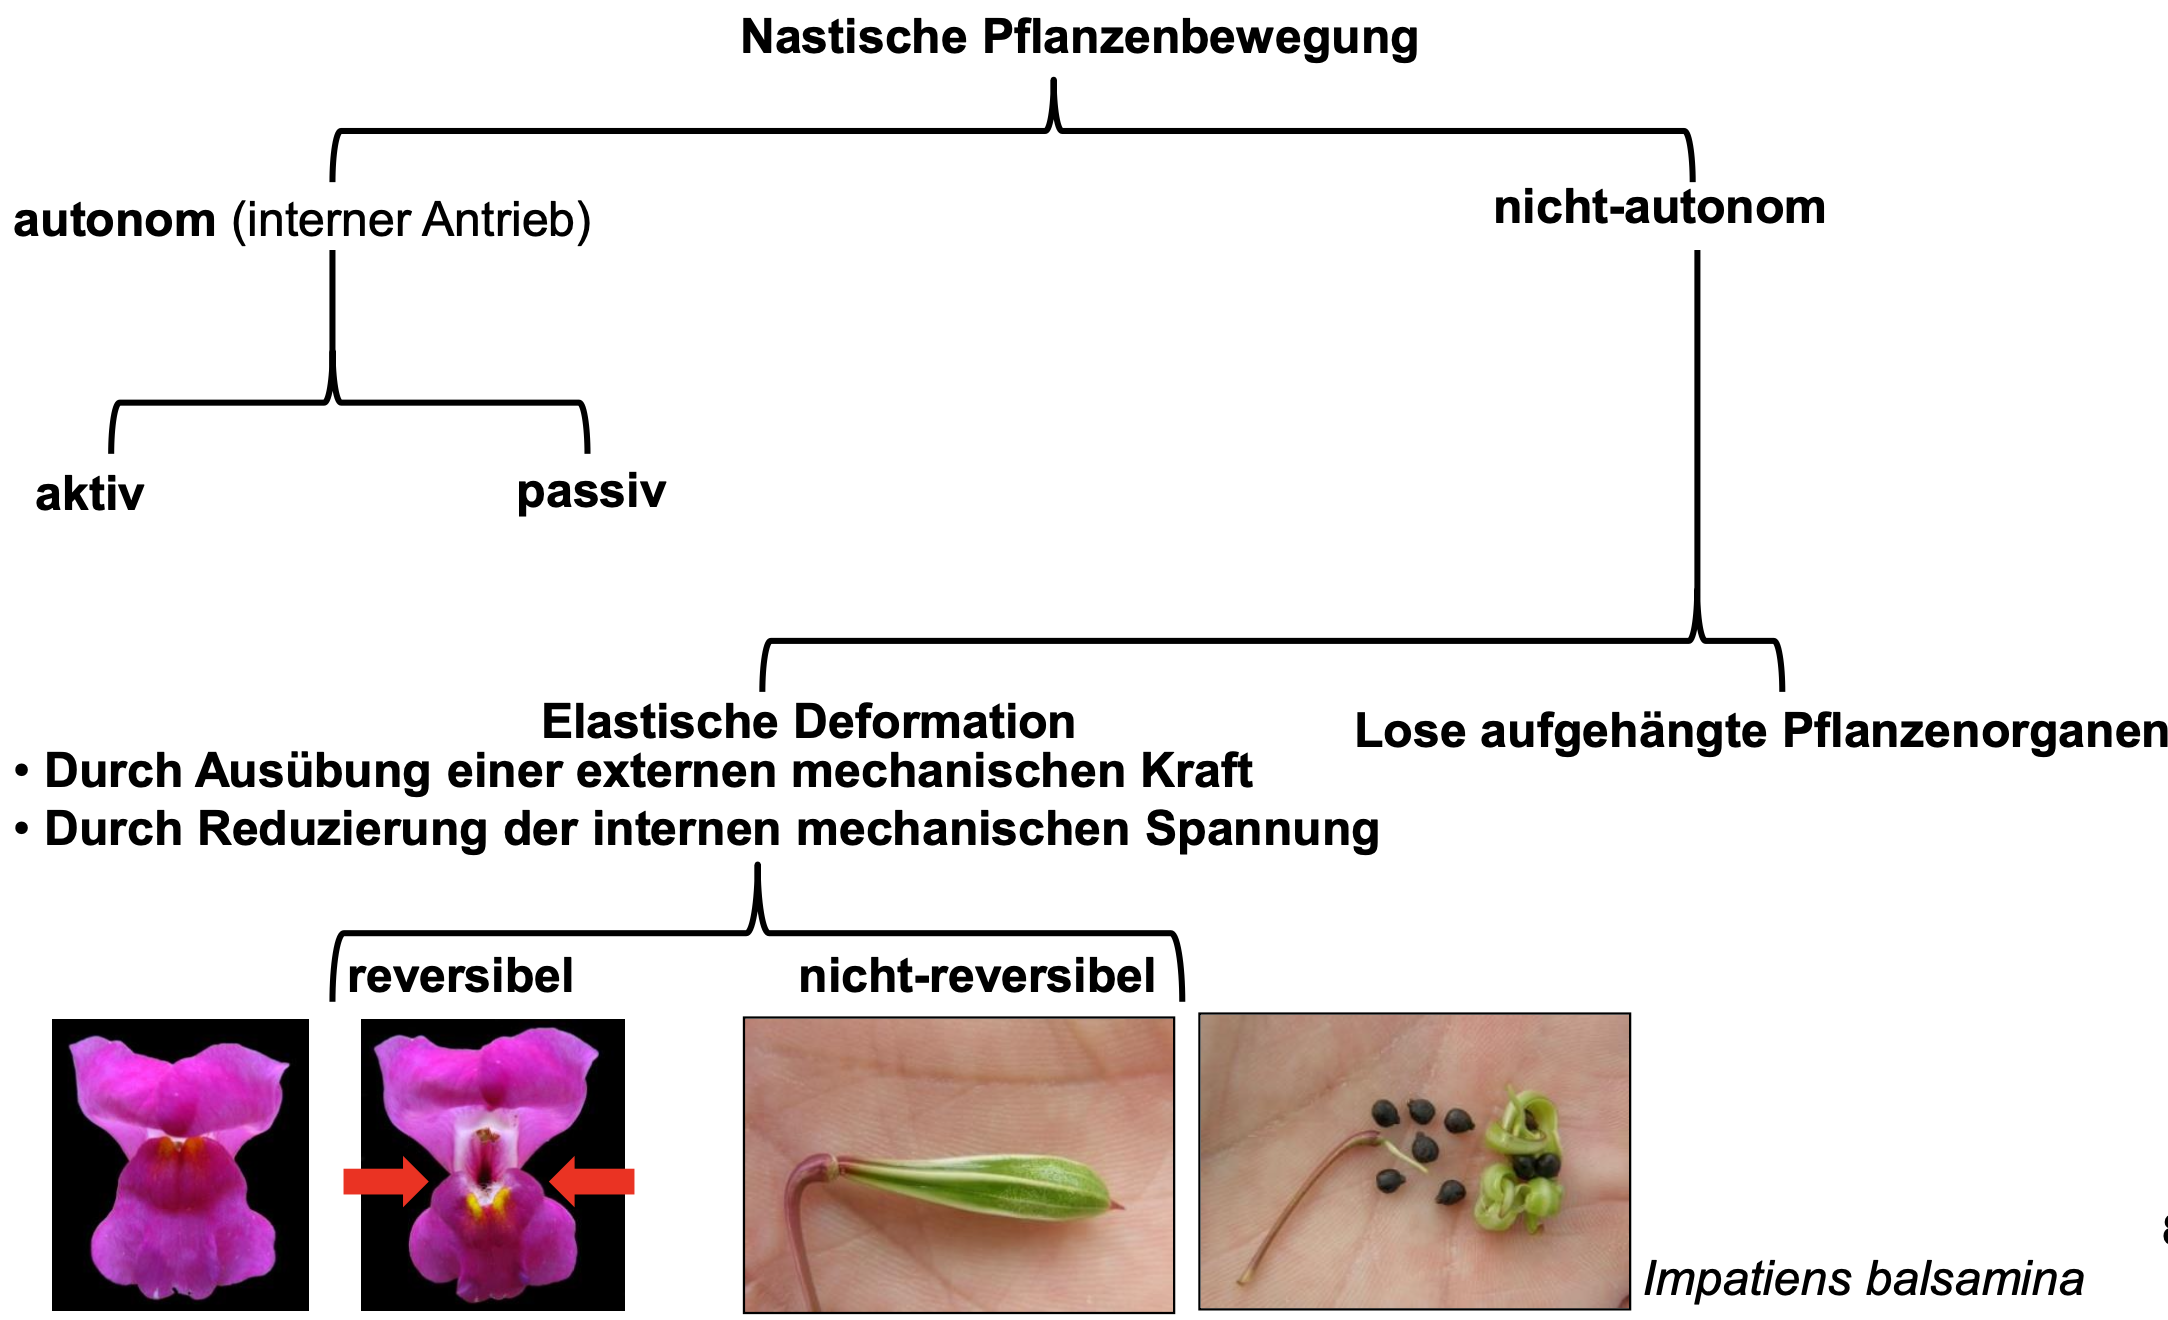
\includegraphics[width=13cm]{lec7/figures/pflanzenbewegung.png}
\end{center}
Viele Pflanzen haben sich in Koevolution auf einen bestimmten Bestäuber angepasst. Ein Beispiel ist eine \textbf{Paradisvogelblume (Strelitzia), die Nektar und Pollen freigibt, wenn ein Vogel sich auf eine Stange an der Blütenkrone setzt} \dangersign. In der Natur dient dies zum Schutz des Blütenstaubs.

\textit{Bionische Anwendung} \dangersign: Eine elastisch deformierbare Sonnenblende, die bei Schub an einem Ende ihre Fläche um 90° zur Seite faltet. Mögliche Anwendung zur außenliegenden Fassadenverschattung.

\begin{center}
    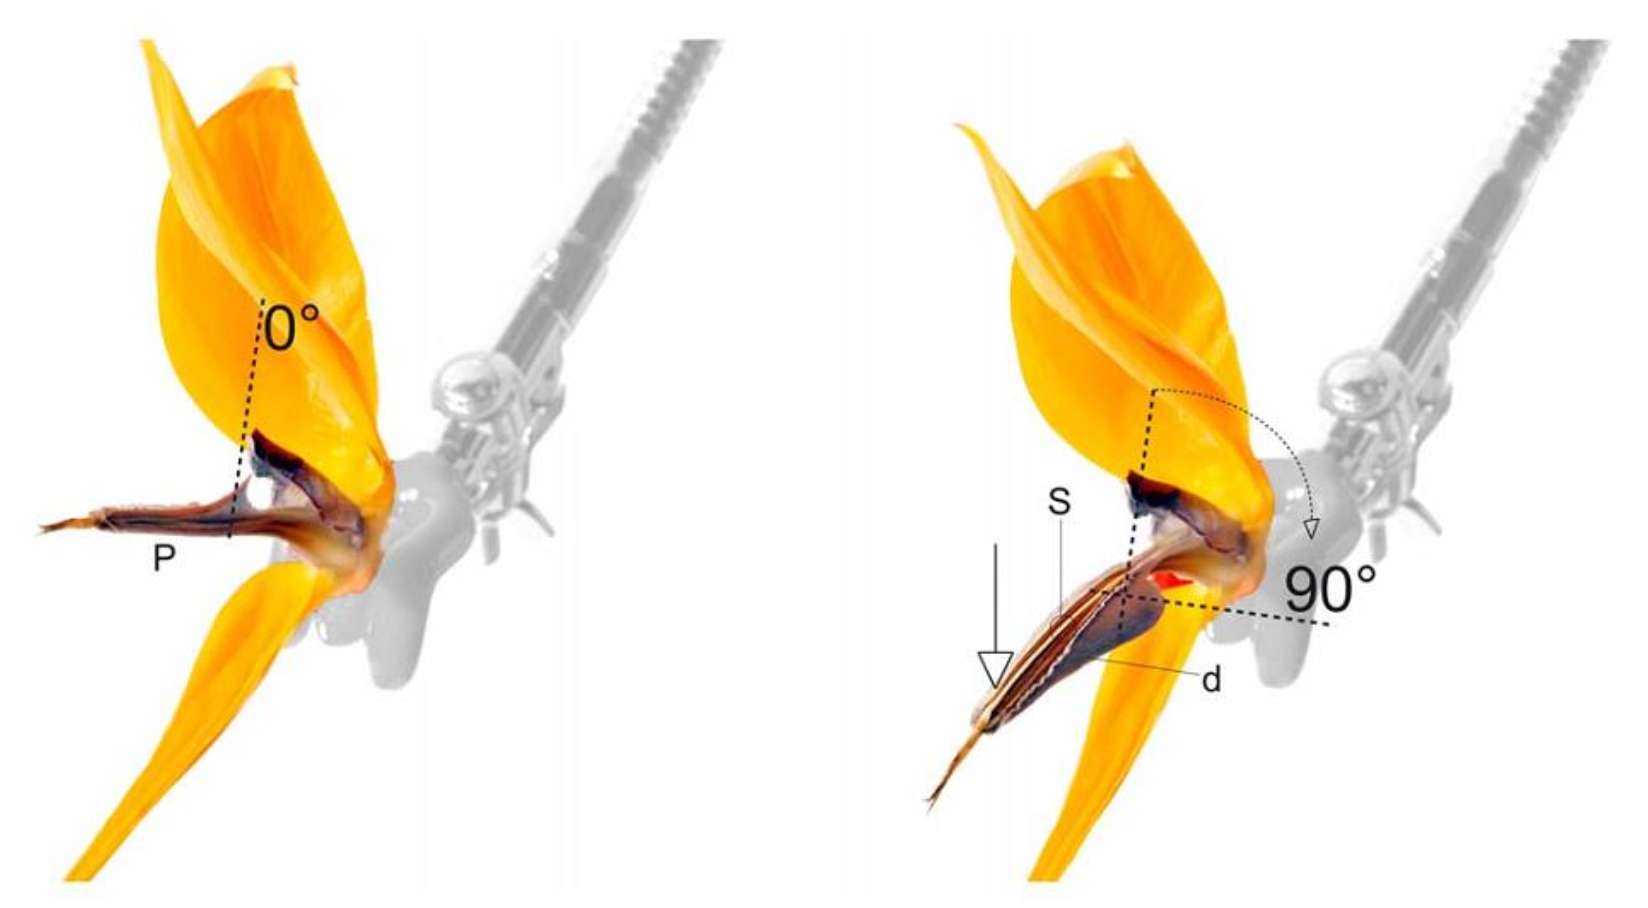
\includegraphics[width=6cm]{lec7/figures/stange.png}
    \hfill
    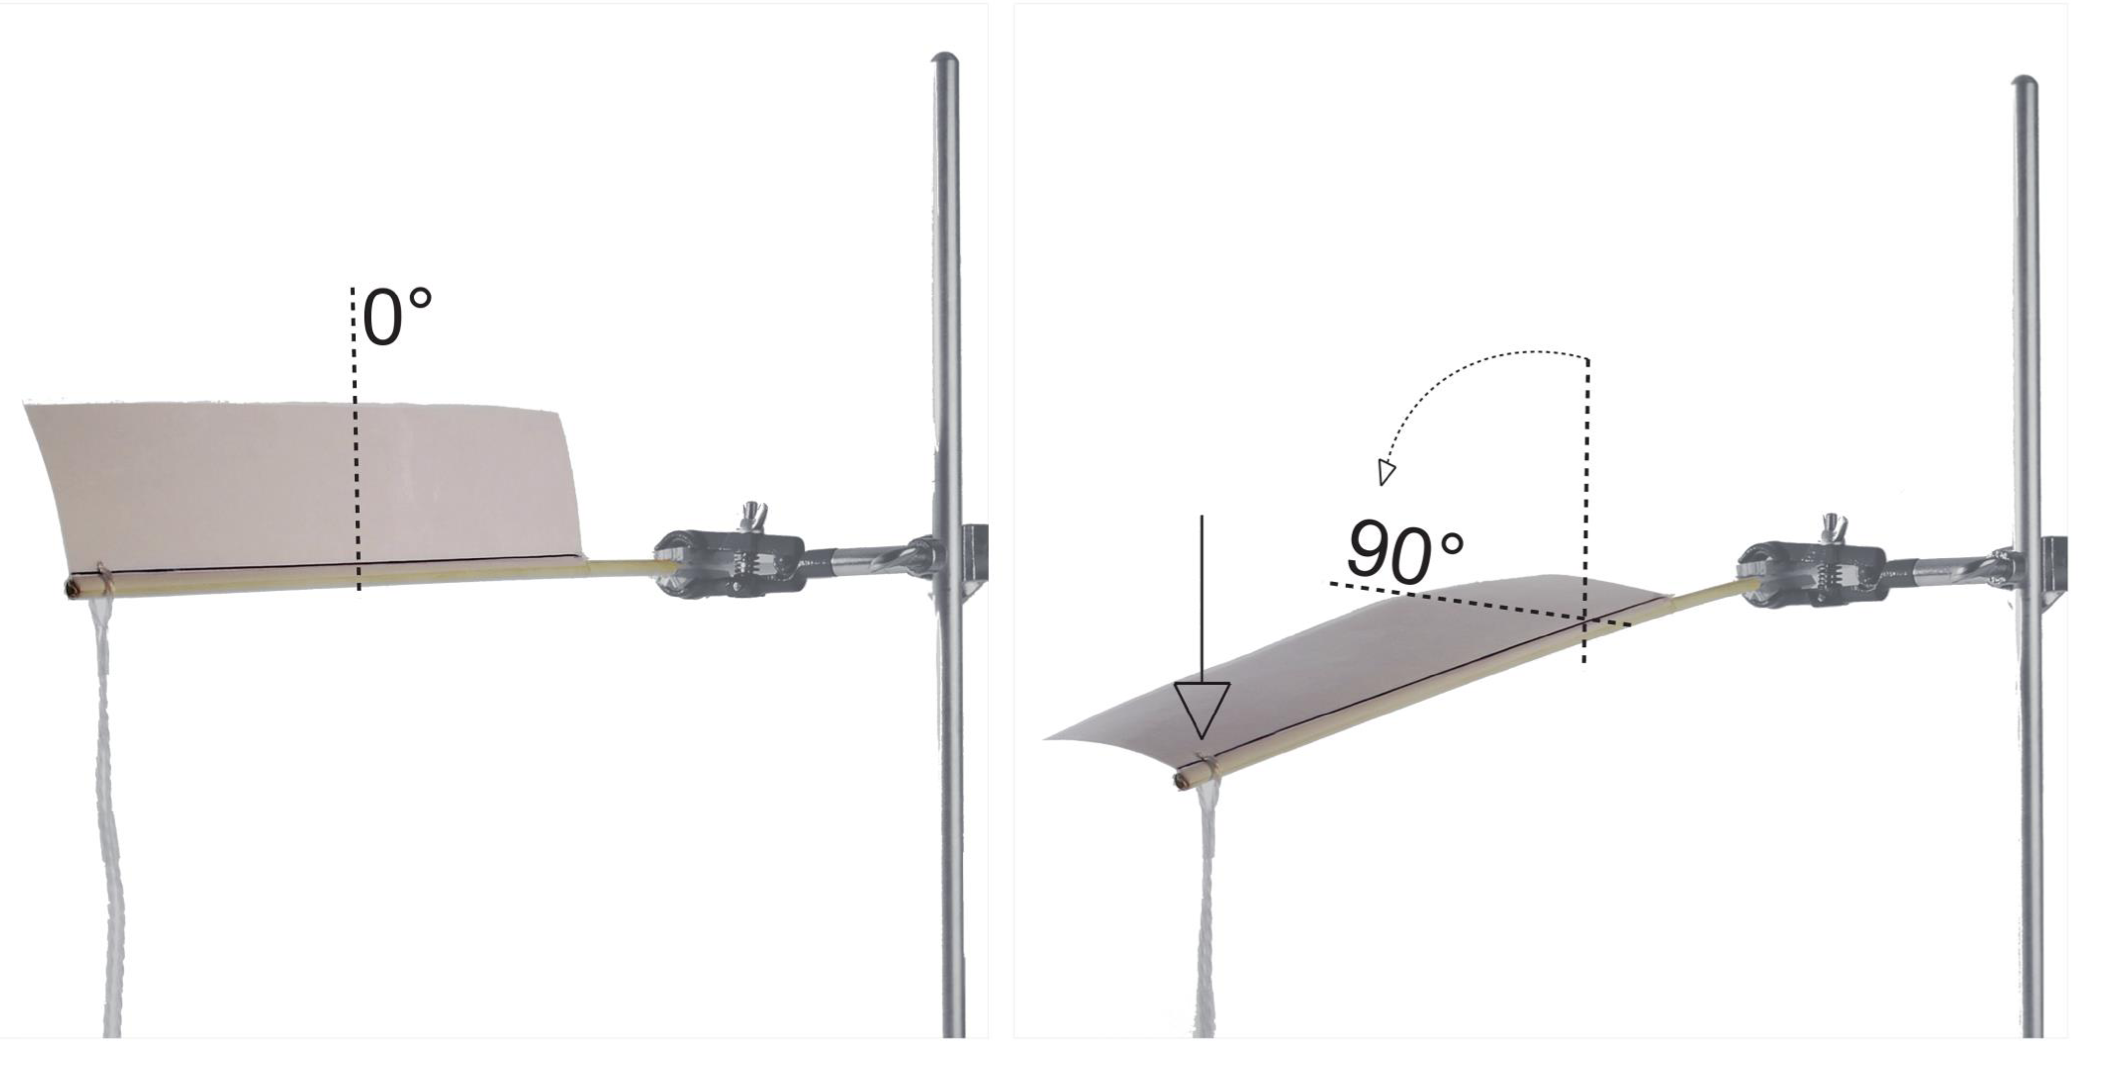
\includegraphics[width=6cm]{lec7/figures/stange_bio.png}
    \hfill
    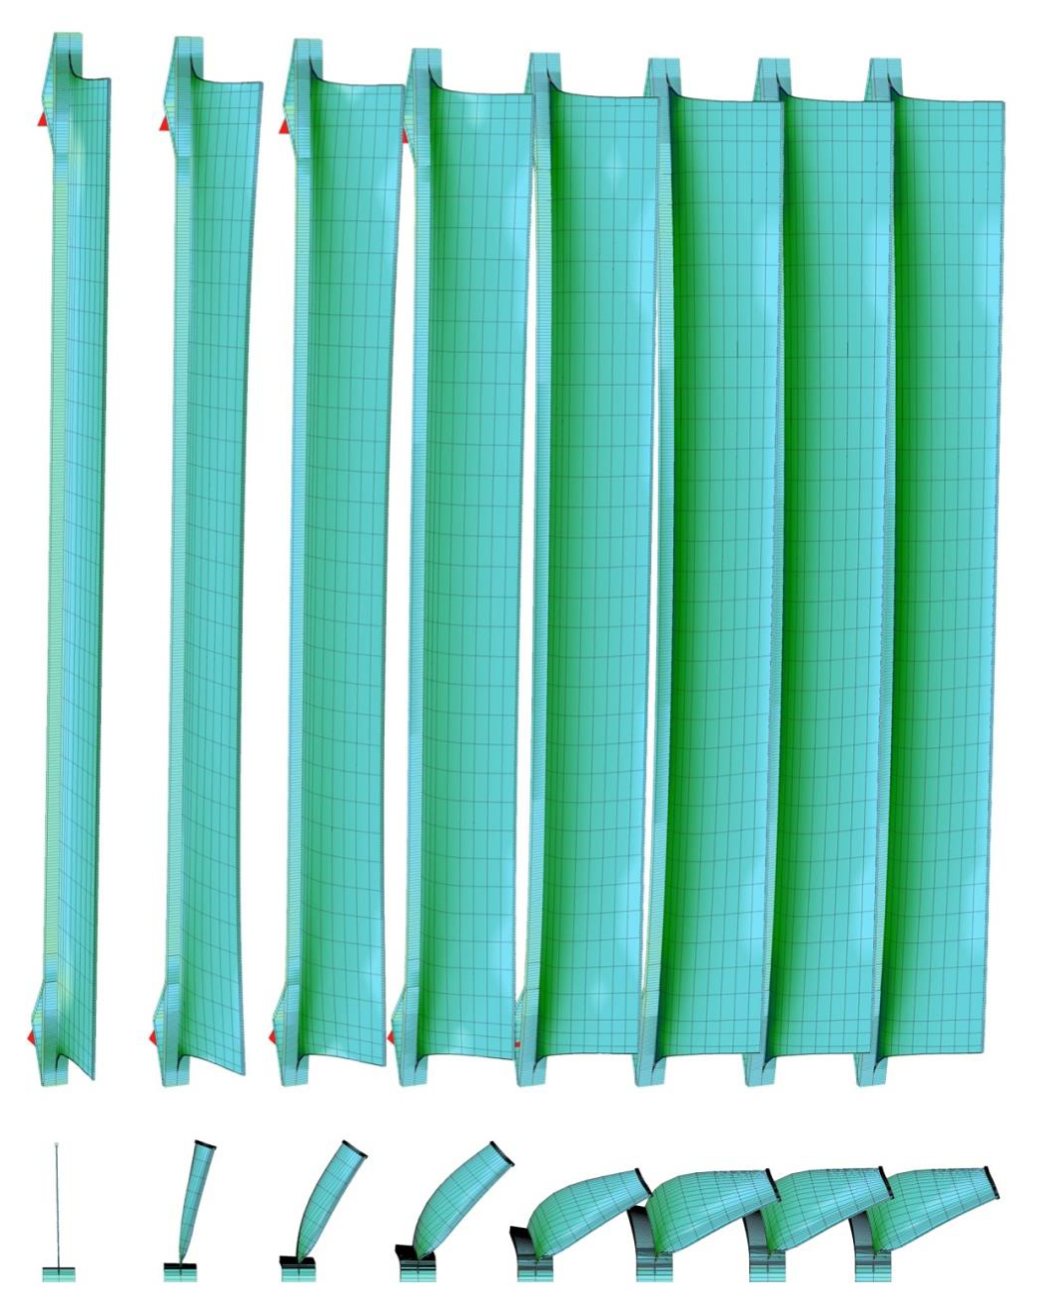
\includegraphics[width=3cm]{lec7/figures/sonnenblende.png}
\end{center}

\subsubsection{Das Eisbärfell als transparentes Isoliermaterial}

Jedes Haar vom Eisbären einthält einen schwarzen Zentralzylinder (``Haarmark'') mit Strukturen (``Streuzentren'') die das Licht streuen. Dieses \textbf{Streulicht lässt die Haare weiß erscheinen}. Weil das Haar zylindrisch gebaut ist wird das Licht aufgrund von Totalreflexion im Haar gehalten. Zudem wird \textbf{kurzwelliges Licht durch Lumniszenz in Wärmestrahlung umgewandelt und dann durch die dunkle Haut aufgenommen} \dangersign. Weiterhin bilden die Haare im Fell eine Vielzahl von luftgefüllten Zwischenräumen
und unterstützen daduch die Wärmeisolation \dangersign.

\textit{Bionische Anwendung als Transparentes Isoliermaterial.} Vorteil:
Streuung des Lichts führt zu blendfreier Bürobeleuchtung

\begin{center}
    \includegraphics[width=8cm]{lec7/figures/eisbär.png}
\end{center}

\subsubsection{Klimaregelung im Termitenbau}

Termitenstaaten bestehen aus mehreren Millionen Individuen und einige Termitenarten kultivieren Pilze in ihren Bauten. Sowohl diese Pilze als auch die Termiten haben gewisse Ansprüche an die Menge an $CO_2$ und $O_2$, sowie die Temperatur im Bau. Es werden deshalb Lüftungsmechanismen eingebaut und die Bauten nach der Sonneneinstrahlung ausgerichtet. 

\textbf{Die Klimaregelung funktioniert folgendermaßen \dangersign:} Kaminartige Strukturen
führen bei starker Erwärmung durch Sonneneinstrahlung zum Aufsteigen von warmer Luft im Bau. Es entsteht ein Unterdruck der kühle Luft aus tieferen kühlen Gängen ansaugt (z.T. in Kontakt mit Grundwasser). Bei extremen Bedingungen verändern die Termiten den Kaminquerschnitt aktiv durch Anlagerung / Abtragung von Baumaterial.

\begin{center}
    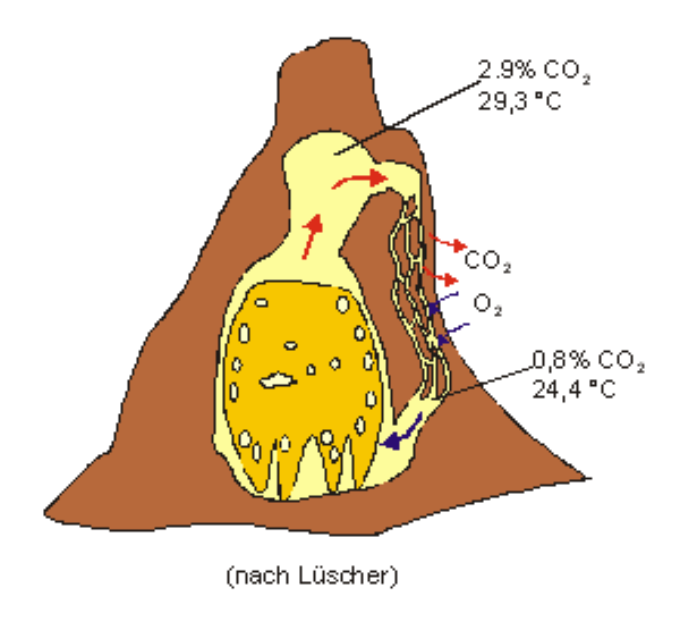
\includegraphics[width=8cm]{lec7/figures/termiten.png}
\end{center}
\textit{Bionische Umsetzung:} Lüftungskamine der Universität Leicester, wobei der Stromverbrauch um 50\% reduziert wurde. Allerdings sind diese Systeme weiterhin nicht passiv.
 

